%%%%%%%%%%%%%%%%%%%%%%%%%%%%%%%%%%%%%%%
%%%%%%%%%%%%%%%%%%%%%%%%%%%%%%%%%%%%%%%

\begin{abstract}

Meiotic recombination in mammals has been shown to largely cluster into hotspots, which are targeted by the chromatin modifier PRDM9.
The canid family, including wolves and dogs, has undergone a series of disrupting mutations in this gene, rendering \textit{PRDM9} inactive.
Given the importance of \textit{PRDM9} it is of great interest to learn how its absence in the dog genome affects patterns of recombination placement.
We have used genotypes from domestic dog pedigrees to generate sex specific genetic maps of recombination in this species.
On a broad scale, we find that placement of recombination events in dogs is consistent with that in mice and apes, in that the majority of recombination occurs toward the telomeres in males, while female crossing over is more frequent and evenly spread along chromosomes.
It has been previously suggested that dog recombination is more uniform in distribution than that of humans,
however, we found that recombination in dogs is less uniform than humans. % and that this effect is stronger in males of both species.
We examined the distribution of recombination within the genome, and 
find that recombination is elevated immediately upstream of the transcription start site, and around CpG islands, in agreement with previous studies, but find that this effect is stronger in male dogs.
We also find evidence for positive crossover interference influencing the spacing between recombination events in dogs, as has been observed in other species including humans and mice.
Overall our data suggests that dogs have similar broad scale properties of recombination to humans,
while fine-scale recombination is similar to other species lacking \textit{PRDM9}.

\end{abstract}


\section{Introduction}

The placement of recombination events within the genome is not random but instead is concentrated into regions known as hotspots. % (in most eukaryotes).
Recent work has identified the protein PRDM9 as responsible for targeting recombination events to hotspots\cite{Baudat2010,Myers2010,Parvanov2010}.
PRDM9 is active early in meiotic prophase\cite{Hayashi2005} and contains a zinc finger (ZF) array that binds to specific DNA motifs located at hotspot centers.
Upon DNA binding, PRDM9 trimethylates lysine 4 on histone H3, and is presumed to recruit cellular machinery to initiate recombination through an unknown mechanism.

Recombination hotspots are a common feature of eukaryote genomes but are not typically conserved between species.
For example, humans and chimpanzees have a complete absence of hotspot sharing, despite a high degree of overall DNA sequence identity\cite{Ptak2005,Winckler2005,Auton2012a}.
This change in hotspot location appears to be driven by the rapid evolution of the
ZF domain of \textit{PRDM9}, which is subject to strong selection in primates and rodents as well as a variety of ancient metazoans\cite{Oliver2009}.
Alterations to the ZF domain modify DNA motif recognition and binding specificity\cite{Oliver2009}
and hence contribute to a shifting landscape of active hotspots in the genome.

Evidence suggests that PRDM9 is required for the proper completion of meiosis.
Loss of \textit{PRDM9} causes sterility in male mice due to impairment of the progression of early meiotic prophase\cite{Hayashi2005}.
These mice, despite being sterile, still initiate double strand breaks (DSBs), and these breaks cluster into hotspots.
However, there is almost no overlap with hotspots that occur in mice with functional PRDM9, and these DSBs occur preferentially at promoters and CpG rich regions of the genome\cite{Brick2012}.  %away from sites of H3K4 trimethylation
%Despite the absence of PRDM9 in the dog genome, crossovers still cluster into hotspot-like regions, and these tend to be CpG rich regions that occur near gene promoters\cite{Axelsson2012,Auton2013}.
This pattern is similar to that in other species lacking \textit{PRDM9}, including birds\cite{Singhal2015}, and yeast\cite{Lam2015}. %, and knockout mice\cite{Brick2012}.

The canid orthologue of \textit{PRDM9} has been inferred to have undergone multiple truncating mutations in the last exon, encoding the ZF array, and become a nonfunctional pseudogene\cite{Munoz-Fuentes2011}.
These mutations are shared within the Canidae family that includes dogs, coyotes, wolves, and foxes and must have accumulated after their divergence from pandas, who do not share the mutations, approximately 49 Mya\cite{Oliver2009,Munoz-Fuentes2011,Axelsson2012,Auton2013}.
Nonetheless, these species are all able to complete meiosis and reproduce,
which implies either that the function of PRDM9 in dogs is replaced by another gene or that recombination is able to complete successfully in its absence.
A rare homozygous loss of function mutation in \textit{PRDM9} has been recently reported in humans, in which a healthy mother was found to have mutations predicted to abolish both methlytransferase and DNA binding activity\cite{Narasimhan2016}, leading to 
 reduced crossover activity at PRDM9-dependent hotspots.
Transmission of the mutation was detected in one of her three healthy children, suggesting that humans may be able to successfully complete meiosis and remain fertile without functional PRDM9.

Despite the lack of \textit{PRDM9}, hotspot-like regions of recombination have been inferred in dogs from patterns of linkage disequilibrium (LD).
These hotspots differ qualitatively from those found in humans, appearing to have a lower intensity of recombination rate, and covering a wider genomic interval ($\sim$4-18 kb compared with $\sim$2 kb in humans)\cite{Axelsson2012,Auton2013}.
However, direct comparisons are complicated by differences in the general LD properties of the species arising from, for example, population demography\cite{Auton2013}.
%Fewer hotspots were detected in dogs, potentially due to a lowered intensity combined with reduced statistical power.
Most striking is the observation that recombination is preferentially targeted towards CpG rich regions, such as those found in gene promoter regions,
which is similar to recombination patterns found in other species without \textit{PRDM9}.
%The identified hotspots showed a high degree of overlap with gene promoter regions, with 50\% of hotspots occurring within 15 kb and only 17\% occurring more than 100 kb away from transcription start sites (TSS)\cite{Auton2013}.  
%This observation echoes that found in PRDM9 knockout mice, in which DSB hotspots still occur and cluster in CG-rich regions\cite{Brick2012}.


%%% Uniformitivity of recombination in dogs vs humans

Over the last three decades, the study of recombination in dogs has progressed from initial low-coverage linkage maps\cite{Mellersh1997,Neff1999}, bolstered by the assembly of a draft sequence of the dog genome\cite{Lindblad-Toh2005}, to higher-coverage pedigree maps\cite{Wong2010}, and high-resolution LD based maps from single nucleotide polymorphism (SNP) array and whole genome sequence data\cite{Axelsson2012,Auton2013}.
Here, we present a pedigree analysis of recombination in the domestic dog, \textit{Canis lupus familiaris}, using high-density SNP microarray data, which allows investigation of the sex-specific distribution of recombination in the dog genome.
Given the open questions regarding the role of PRDM9 in recombination, we compared the sex-specific landscape of recombination in the dog genome to that inferred from human pedigrees, and used this comparison to gain further insight into the effects of the presence or absence of PRDM9 on the mammalian recombination landscape.
%%%% In general, the results of our study suggest ...

%%%%%%%%%%%%%%%%%%%%%%%%%%%%%%
%%%%%%%%%%%%%%%%%%%%%%%%%%%%%%
\section{Methods}
%%%%%%%%%%%%%%%%%%%%%%%%%%%%%%
%%%%%%%%%%%%%%%%%%%%%%%%%%%%%%

\paragraph{Genotyping.}
The full dataset is derived from genomic analysis of 237 DNA samples, with 25 founder individuals (15 male, 10 female, pedigree structure shown in Figure \ref{fig:pedigree}) from a colony of Labrador Retriever and Greyhound crosses maintained at Cornell University for over 30 years\cite{Todhunter2003}.
Genotyping was performed using genomic DNA as described in \citet{Hayward2016} using Illumina CanineHD BeadChips that include more than 170,000 SNPs. 
All positions reported are given in canFam3.1 coordinates.

% \paragraph{Pedigree splitting.}
% In order to reduce the complexity, we broke up the data into smaller nuclear families.
% In most cases we could identify full phased meioses by using single generation families (21 total), however in two families we could gain additional data by adding grandparents or children from another generation.
% We split the larger single generation familes further, so that none had more than 9 children (corresponding to a bit size of 16).
% Following recombination event calling, the larger pedigrees were rejoined for further analysis.


\paragraph{Filtering SNP data.}
To avoid spurious recombination calls due to genotyping error, we applied a set of filters on the variant data (outlined in Figure \ref{fig:pipeline}).
First, 586 SNPs were removed because they had missing genotypes in greater than 5\% of the samples.
We then used the PLINK\cite{Purcell2007} software (v1.07) to identify and remove a further 1,245 SNPs showing Mendelian errors in transmission (option \verb|--mendel|).
The error detection feature in the Merlin\cite{Abecasis2002} software (v1.1.2, option \verb|--error|) was used to identify and remove SNPs with genotypes that conflicted with pedigree structure and are likely to be genotyping errors.
Three iterations of Merlin error detection were performed, removing 1,363, 66, and 7 SNPs, respectively.
In total 2,771 unique SNPs were filtered out in the first round, leaving 163,400 SNPs for further analysis.

\paragraph{Calling crossover events.}
Autosomal recombination events were inferred using a combination of software tools.
First, the dog genomes were phased without using pedigree information using SHAPEIT2\cite{Delaneau2013} (v2.r790).
In order to avoid bias in our inference of recombination, we use a map file for phasing that has a constant rate of recombination (1 cM/Mb) between physical markers.
Following phasing, we used the duoHMM\cite{OConnell2014} software (v0.1.4) to call recombination events using a hidden Markov model approach.
%Next the duoHMM\cite{OConnell2014} software (v0.1.4), which first phases the genome in the absence of pedigree information using SHAPEIT2\cite{Delaneau2013},
The first duoHMM pass integrated pedigree structure information to correct phasing errors.
Then, duoHMM was used to call crossovers in each parent-child duo of the pedigree, of which only high-confidence events were retained (with probability $>$0.5).
The duoHMM method was also used to identify SNPs that have a high probability of genotyping error (which we removed if a SNP had a probability of error of $>$0.9).
This method has been demonstrated to have a high sensitivity and low false discovery rate when compared to a standard Lander-Green\cite{Lander1987} approach, such as that implemented in Merlin\cite{Abecasis2002}.

% Upon examination of the initial genetic maps generated from the duoHMM crossover calls we identified several regions that exhibited biologically unrealistic recombination rates within concentrated physical regions and could be errors.
% Closer inspection revealed that several regions overlap previously identified structural variants\cite{Nicholas2009,Chen2009}, which could account for the observed clustering of crossovers.
% Another possible explanation is that the reference genome contains misplaced or inverted contigs within these regions, which would lead to calling of false crossover events on either side of the out of place region.
% We removed all 435 variants within four such regions, totaling 5.6 Mb of sequence (Table \ref{tab:badregions}).
% A further 1,344 markers were removed using the error detection feature of duoHMM (with a probability of error of 0.9 or higher).

% After this second round of filtering the dataset consists of 161,699 markers.
% The duoHMM pipeline was then re-run, resulting in 8,312 autosomal recombination events with probability greater than 0.5.
% We observed a number of tight double-crossovers within individuals, which could occur naturally as a result of gene conversion.
% However, in many cases these double crossovers are found to belong to a shared parent, and are further clustered into similar regions of the genome, often using the same SNP for the interval boundaries, strongly suggesting genotyping error as a likely cause.
% We therefore remove any double crossovers if they are found to cluster within 1 Mb, and if more than one meiosis transmitted from the same parent also has clustered crossovers with shared interval boundaries.
% This excluded 90 events out of a total of 8,312 (1.1\%).

% Finally, we excluded meioses that have a biologically abnormal number of crossovers.
% We excluded meioses more than 4 standard deviations from the sex-specific median crossover count, with the standard deviation estimated via the robust estimator of 1.4826 MAD (median absolute deviation).
% In females, we exclude 3 meioses (with 55, 41, and 119 crossovers) exceeding a cutoff of 39, and none under the lower bound of 4.
% In males, we exclude 1 meiosis (with 5 crossovers) under the lower bound of 6, and 2 meioses (with counts of 44 and 109) above 29 crossovers.

% \paragraph{Summary of filtered dataset.}
% The filtered dataset consists of 408 informative meioses, 204 from females, and 204 from males, and
% a total of 7,849 well supported crossover events identified across the 38 autosomes.
% %Crossovers can be localized to a region of uncertainty bounded by flanking heterozygous markers in the parent.
% %The distribution of interval sizes is show in Figure \ref{fig:intsize} and can be resolved to a median size 102.1 kb.

% Following removal of weakly-supported SNPs, we use Merlin to reconstruct haplotypes within each nuclear family (option --best) and identify recombination events.
% We first remove 1661 events with zero informative sites on either side of the interval.
% An informative site is defined for a parent-child trio and must be heterozygous in the parent in which the meiosis occurs, and heterozygous in either the other parent or the child.
% Next, we exclude 210 events that occur more than 2 times in the same SNP interval in the same family.
% Finally, 48 events were removed that clustered within 1 Mb in each pedigree.
% From an initial set of 9754 crossovers, these filters remove 1919 events, leaving 7835 for further analysis.
% Of these filtered events there were 4038 female and 3656 male events in the 38 autosomes, a female to male ratio of 1.10, slightly lower than the 1.19 ratio previously reported in dogs\cite{Wong2010}.

\paragraph{Filtering crossovers.}
Tightly clustered crossovers within individuals may occur naturally as a result of gene conversion, however another possibility is that genotype errors have caused false crossover calls.
In many cases in our data we found double crossovers that belonged to a shared parent, and are clustered within the genome.
Furthermore, these crossovers often used the same SNP for the interval boundaries.
This strongly suggests genotyping error as a likely cause.
We therefore removed any double crossovers if that cluster within 1 Mb, and if more than one meiosis transmitted from the same parent also has clustered crossovers with shared interval boundaries.

We further remove all crossovers attributed to meioses that have biologically abnormal crossover counts.
We define thresholds separately for males and females, with a distribution centered around the median crossover count, and defining the boundaries as 4 standard deviations from the sex specific median crossover count, with the standard deviation estimated via the robust estimator of 1.4826 MAD (median absolute deviation).
%In females, we exclude 3 meioses (with 55, 41, and 119 crossovers) exceeding a cutoff of 39, and none under the lower bound of 4.
%In males, we exclude 1 meiosis (with 5 crossovers) under the lower bound of 6, and 2 meioses (with counts of 44 and 109) above 29 crossovers.

\paragraph{Construction of the genetic map.}
Due to the high level of inbreeding and homozygosity in domestic dogs,
it is often not possible to detect recombination events over a significant fraction of the genome within a given pedigree.
For example, if a breeding pair have few heterozygous variants towards the telomeric ends of a given chromosome, then events occurring within such regions will be largely invisible as they will not be flanked by informative markers.
Due to the high level of inbreeding within many dog samples, failure to account for this issue would result in an underestimate of the total map length.
To correct for this issue, we considered the location of informative markers within each pedigree, and scaled the genetic map accordingly.

In order for duoHMM to correctly identify a recombination event, it must be flanked by at least one heterozygous variant in the parent on each side.
%Crossovers that occur near the chromosome end and past the most extreme heterozygous marker are more likely to be missed by our analysis.
%This has the effect of lowering the total number of observed meioses in such regions.
For each parent-child duo for which we are able to make crossover calls, we identified the positions of the first and last heterozygous variant on each chromosome, which represent the genomic range in which we are able to observe a crossover.
Then, across all duos in our sample, we estimated the effective total number of meioses at each position along each chromosome (Figure \ref{fig:mstep}).
The effective number of meioses was used in place of a fixed number of meioses when calculating the recombination fraction at each genomic interval.

Recombination fractions were converted to genetic distances using Haldane's map function.
Comparing maps generated using the effective number of meioses to those using a fixed number of meioses, we observed an increase in autosomal map length for both females (59.7 cM) and males (49.2 cM), and an increase in the sex averaged map length of 48.6 cM (Figure \ref{fig:mstepIncrease}).

\paragraph{Estimation of crossover interference parameters.}
Crossover interference influences the spacing of crossover events when two or more occur on the same chromosome in the same meiosis.
We modeled the distance between these crossovers using two models.
The gamma model\cite{Broman2000} assumes that the inter-crossover distances follow a simple gamma distribution with shape $\nu$ and rate $2\nu$, where $\nu$ is a unitless measure of the strength of crossover interference,
with $\nu=1$ representing no crossover interference, $\nu<1$ representing negative interference (spaced closer than expected by chance), and $\nu>1$ indicating positive crossover interference (spaced further apart than expected).
The gamma-escape model, originally proposed by \citet{Housworth2003} provides an extension to the simple gamma model.
Here, crossovers that are governed by the interference effect ($\nu>1$) are modeled to coexist alongside a subset of crossovers that escape interference ($\nu=1$).
A second parameter, $p$, is included to allow the second class of ``escaping'' crossovers to exist in a mixture with the interfering crossovers, and represents the proportion of events that escape interference.
To measure crossover interference, we estimated the parameters $\nu$ and $p$ using a MATLAB software package (\url{https://github.com/auton1/interference}) previously developed to analyze interference in humans\cite{Campbell2015}.

In order to compare each of the fitted models, we used the Bayesian Information Criterion (BIC), which is given by:
$BIC = -2 \ln( L ) + k \ln( n )$
, where $L$ is the maximum likelihood estimation from the model fit, $k$ is the number of free parameters in the model, and $n$ is the number of observations.
The model with the smallest BIC is preferred.

\paragraph{Gene annotations.}
Gene annotations for canFam3.1 were downloaded from Ensembl (build 81).
We considered only protein coding genes located on the autosomes, and kept the longest isoform for each gene.

\paragraph{Thinning the human map.}
In order to make a valid comparisons between dogs and humans with respect to the proportion of recombination occupying a given amount of sequence, we took a number of steps to ensure the datasets are as similar as possible.
To enable sex-specific comparisons between the species, we used a human pedigree dataset (\citet{Campbell2015}) rather than an LD-based map.
As the human dataset is considerably larger, we randomly sampled 408 phase-known meioses (204 each from males and females) to match the size of the dog dataset.
We then reduced the SNP density of the human data.
The human dataset was genotyped on a microarray of higher density than we have available for dogs, which allows recombination events to be better resolved than what was possible for dogs.
We therefore thinned the human dataset in an attempt to match the recombination event resolution in dogs using an \textit{ad hoc} iterative process as follows: 
1) Determine the inter-SNP distances for the human and dog datasets,
2) find SNPs that cluster more tightly in humans
3) remove a random subset of SNPs within each of these clusters,
4) iterate until the inter-SNP distributions and overall medians are similar between the two species.
This iterative process yields a thinned framework of SNPs in the human dataset such that the new inter-SNP distances closely resemble those in dogs (Figure \ref{fig:interSNPdist}).
Following this thinning, we examined each individual crossover in the human data, and expanded the interval boundaries, if necessary, to the next available SNP in the newly selected framework.
New sex specific genetic maps were then generated from this thinned data and used for the comparison to dogs.

\paragraph{Data availability.}
Supplementary data for this study, including sex-specific genetic maps, filtered crossover calls, and genotype data are available at 
\\ \url{https://github.com/clcampbell/dog_recombination}.

%%%%%%%%%%%%%%%%%%%%%%%%%%%%%%%%%%%%%%%%%%%%%%%%%%
%%%%%%%%%%%%%%%%%%%%%%%%%%%%%%%%%%%%%%%%%%%%%%%%%%
\section{Results}
%%%%%%%%%%%%%%%%%%%%%%%%%%%%%%%%%%%%%%%%%%%%%%%%%%
%%%%%%%%%%%%%%%%%%%%%%%%%%%%%%%%%%%%%%%%%%%%%%%%%%

\paragraph{Building the genetic map.}
We used SNP array genotype data from 237 domestic dogs to map recombination in the canine genome. % generate sex specific genetic maps.
%We performed a series of filtering steps to minimize the amount of genotyping error and ensure high-quality crossover calls in our data set (Figure \ref{fig:pipeline}).
% First, we removed SNPs with a high degree of missing data and that conflict with pedigree structure, indicative of genotyping error.
After applying a series of filtering steps on the SNP data (Figure \ref{fig:pipeline}),
we identified crossovers using duoHMM, a tool previously developed to identify recombination events in human data\cite{OConnell2014}.
Upon examination of the initial genetic maps, we identified several regions that exhibited biologically unrealistic recombination rates within concentrated physical regions and could be errors.
Several of these regions overlap known segmental duplications and copy number variants\cite{Nicholas2009,Chen2009}, which could account for the observed clustering of crossovers.
Another possible explanation is that the reference genome contains misplaced or inverted contigs within these regions, which would lead to calling of false crossover events on either side of the out of place region.
We removed all 435 variants within four such regions, totaling 5.6 Mb of sequence (Table \ref{tab:badregions}), and
a further 1,344 markers identified with the error detection feature of duoHMM. % (with a probability of error of 0.9 or higher).

% After this second round of filtering the dataset consists of 161,699 markers.
%The duoHMM pipeline was then re-run, resulting in 8,312 autosomal recombination events. % with probability greater than 0.5.
After re-calling crossovers on this filtered data, we found 8,312 autosomal recombination events.
We then identified and removed a set of clustered double crossovers, likely to be false calls, consisting of 90 events. % out of a total of 8,312 (1.1\%).
Finally, we excluded meioses that have a biologically abnormal number of crossovers, excluding 3 female meioses (with 55, 41, and 119 crossovers), and 3 male meioses (with 5, 44, and 109 crossovers).
In total we excluded 463 out of 8,312 crossovers (5.6\%).

The filtered dataset consisted of 408 informative meioses, including 204 from females, and 204 from males.
There are 7,849 well supported crossover events that could be localized to a median size of 102.1 kb (Figure \ref{fig:intsize}).
The sex specific genetic maps had a mean resolution of less than 0.4 cM. % 156,318

\paragraph{Comparison to previous studies.}
To assess the accuracy and validity of our results, we compared our maps to those from previous studies.
%We use the sex specific maps generated by \citet{Wong2010} from a pedigree analysis using a combination of microsatellite and low density genome wide SNP data.
%Additionally we use the LD based map from \citet{Auton2013}, based on whole genome sequencing data of 51 village dogs.
We used sex specific maps from a previous pedigree analysis\cite{Wong2010} as well as a sex-averaged LD-based map generated from whole genome sequencing data of 51 village dogs\cite{Auton2013}.
At the broad scale there is close agreement to our sex averaged map from the LD map (Pearson $r=0.86$ at 5 Mb resolution), and from the pedigree sex averaged map ($r=0.75$, Figure \ref{fig:mapCor}A).
% male/female
The male map has a higher agreement with previous studies (LD $r=0.80$, pedigree $r=0.76$, Figure \ref{fig:mapCor}B) than does the female map (LD $r=0.67$, pedigree $r=0.73$, Figure \ref{fig:mapCor}C).

\afterpage{
\begin{table}[p] \centering
    \begin{tabular}{|l|c|c|c|c|c|} 
        \hline Study & Year & Female (cM) & Male (cM) & Ratio & Sex avg.\ (cM) \\ \hline
        Mellersh et al.\cite{Mellersh1997} & 1997 & 1039 & 766 & 1.36 & 902.5 \\
        Neff et al.\cite{Neff1999} & 1999 & 1820 & 1290  & 1.41 & 1555 \\
        Wong et al.\cite{Wong2010} & 2010 & 2276 & 1909 & 1.19 & 2092.5 \\
        Axelsson et al.\cite{Axelsson2012} & 2012 &  &  &  & 3005 \\
        Auton et al.\cite{Auton2013} & 2013 &  &  &  & 2430 \\
        This study & 2016 & 2162 & 1816 & 1.19 & 1978 \\
    \hline \end{tabular}
    \caption{Autosomal map length estimates. Total map lengths are given in centimorgans, while the ratio represents the female to male map lengths. Sex specific map lengths are not available for the LD based maps.\label{tab:mapLengthsSummary}}
\end{table}
\clearpage}

Consistent with previous studies in dogs\cite{Wong2010,Mellersh1997,Neff1999}, and other mammals, including humans\cite{Coop2008,Campbell2015}, females have a longer map length (2162 cM) than males (1816 cM, Tables \ref{tab:mapLengthsSummary} and \ref{tab:mapLengths}).
% ratio
We observed similar total genetic map lengths when compared to the \citet{Wong2010} pedigree study, although our maps are slightly shorter (by 114 cM in females, 93 cM in males, Table \ref{tab:mapLengthsSummary}).
Map length is strongly correlated to physical length in both sexes (male r$^2$=0.82, female r$^2$=0.83), and in the sex averaged maps (r$^2$=0.88; Figure \ref{fig:mapLength}).
The ratio of female to male autosomal map length is 1.19, equivalent to \citet{Wong2010}, but notably lower than that of humans at 1.56\cite{Campbell2015}.

\paragraph{Distribution of recombination.}
%The dog autosome is comprised of 38 acrocentric chromosomes, and we observe a general pattern of low recombination rates near the centromeres and high rates near the telomeres (Figure \ref{fig:recombRate}).
Previous studies showed that the recombination rate is elevated in telomeric regions and lower near the centromere, both in dogs\cite{Wong2010,Axelsson2012,Auton2013}, and other species\cite{DeMassy2013}.
We observed the same phenomenon, and this telomeric effect is largely driven by male recombination in both dogs and humans (Figures \ref{fig:distrRecomb}A, \ref{fig:recombRateHuman}).
The opposite pattern is seen in two chromosomes, 27 and 32, supporting previous evidence\cite{Wong2010} suggesting that the orientation of these chromosomes in the reference genome is likely reversed.
Based on this, we reverse the physical coordinates for these two chromosomes for all further analyses.

We quantified the amount of recombination occurring at the telomeric ends of each chromosome arm by estimating the proportion of total recombination occurring in a physical window located at the telomeric end (Figure \ref{fig:distrRecomb}B).
We found that 38.2\% of recombination occurred within 5 Mb of the telomere in males, compared with 9.7\% in females.
%%% Males show an immediate jump compared to females from the first bin, and at 15\% of the distance from the telomere, male dogs have a much higher proportion of recombination, 47.2\%, occurring in this region, compared to only 18.9\% in females.
Human males have a roughly equivalent proportion within this same region (30.2\% within 5 Mb), while human females have a similar amount of recombination compared to female dogs (7.4\% within 5 Mb).
We conclude that, at a broad scale at least, the telomeric enrichment of recombination observed in male dogs is similar to that of humans.
%, and that males have an enrichment of recombination at the telomeric ends.

\afterpage{
\begin{figure}[p]
    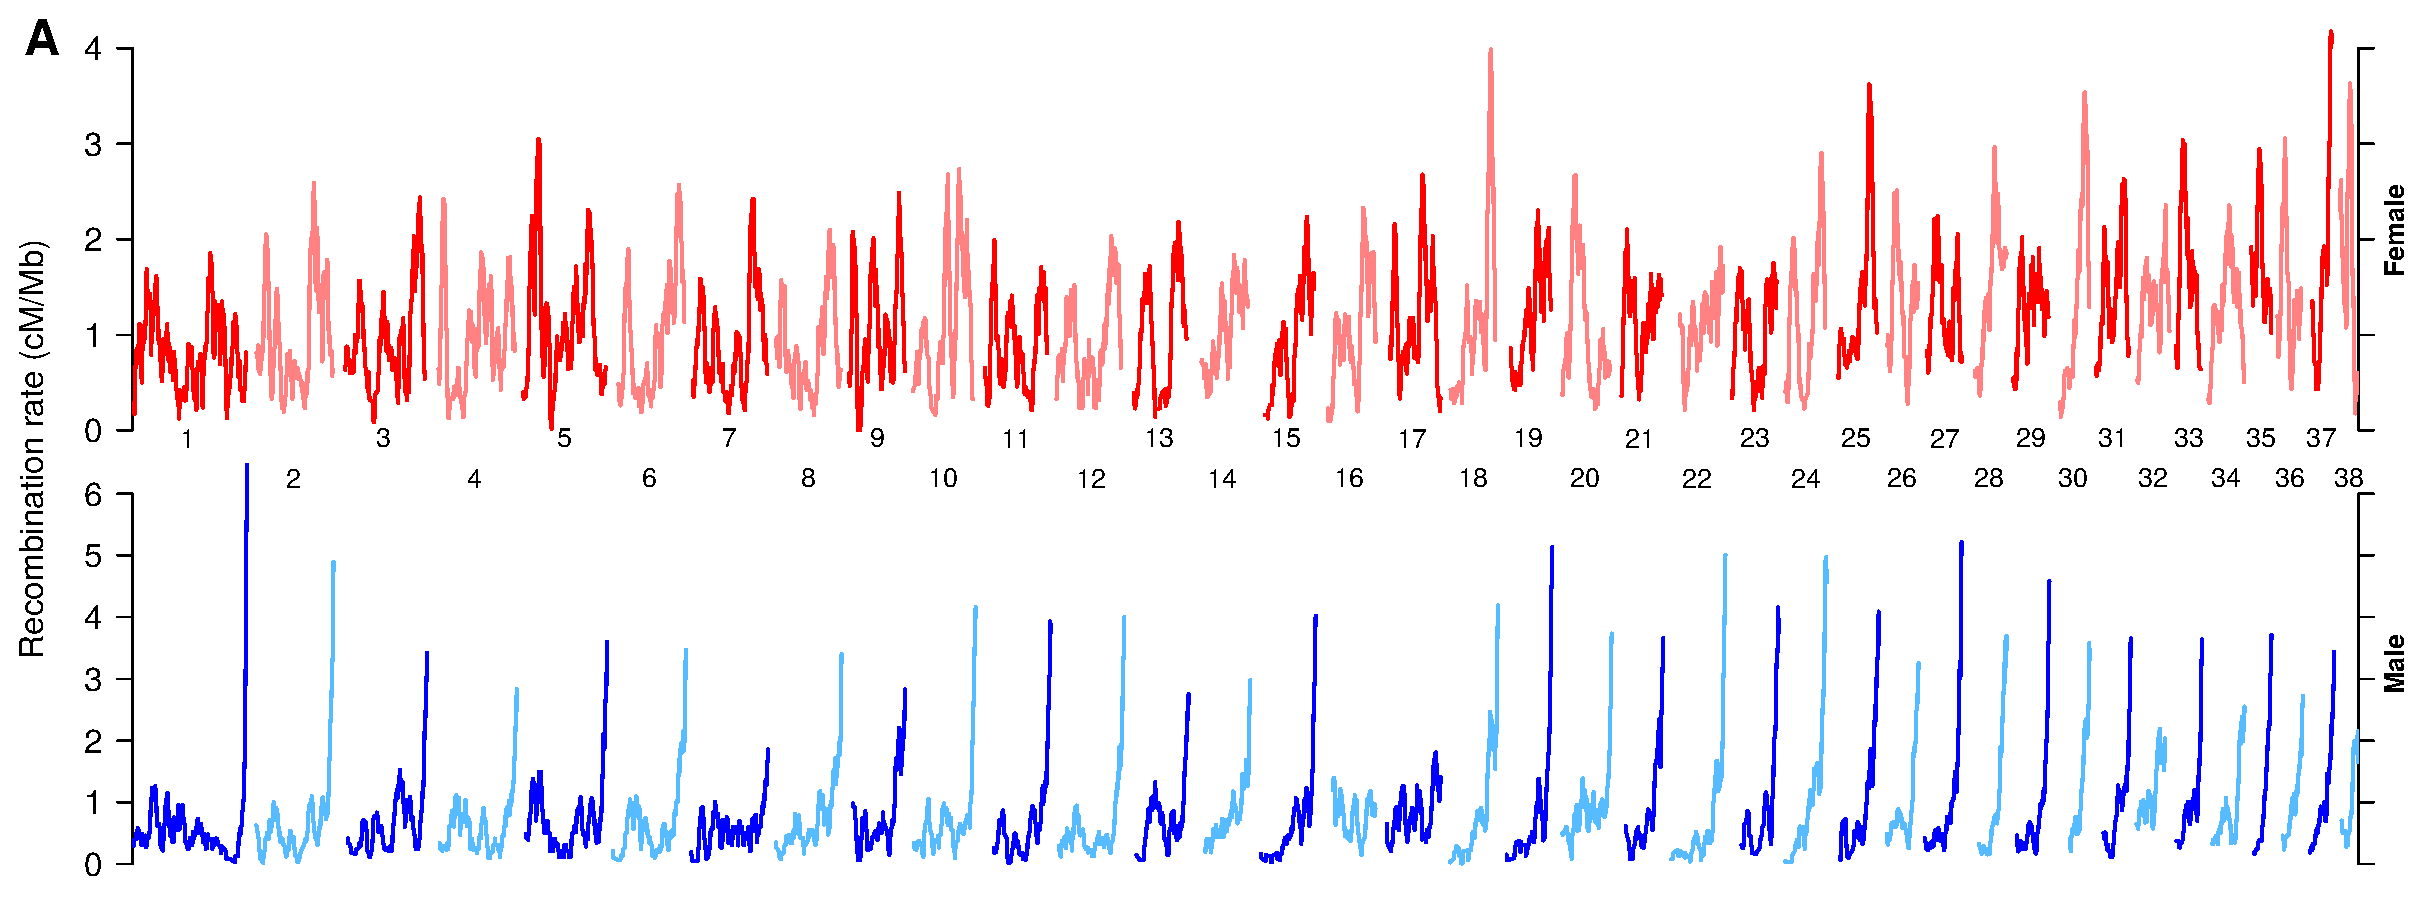
\includegraphics[width=\textwidth]{dogPed/figs/recomb_genome_dog}
    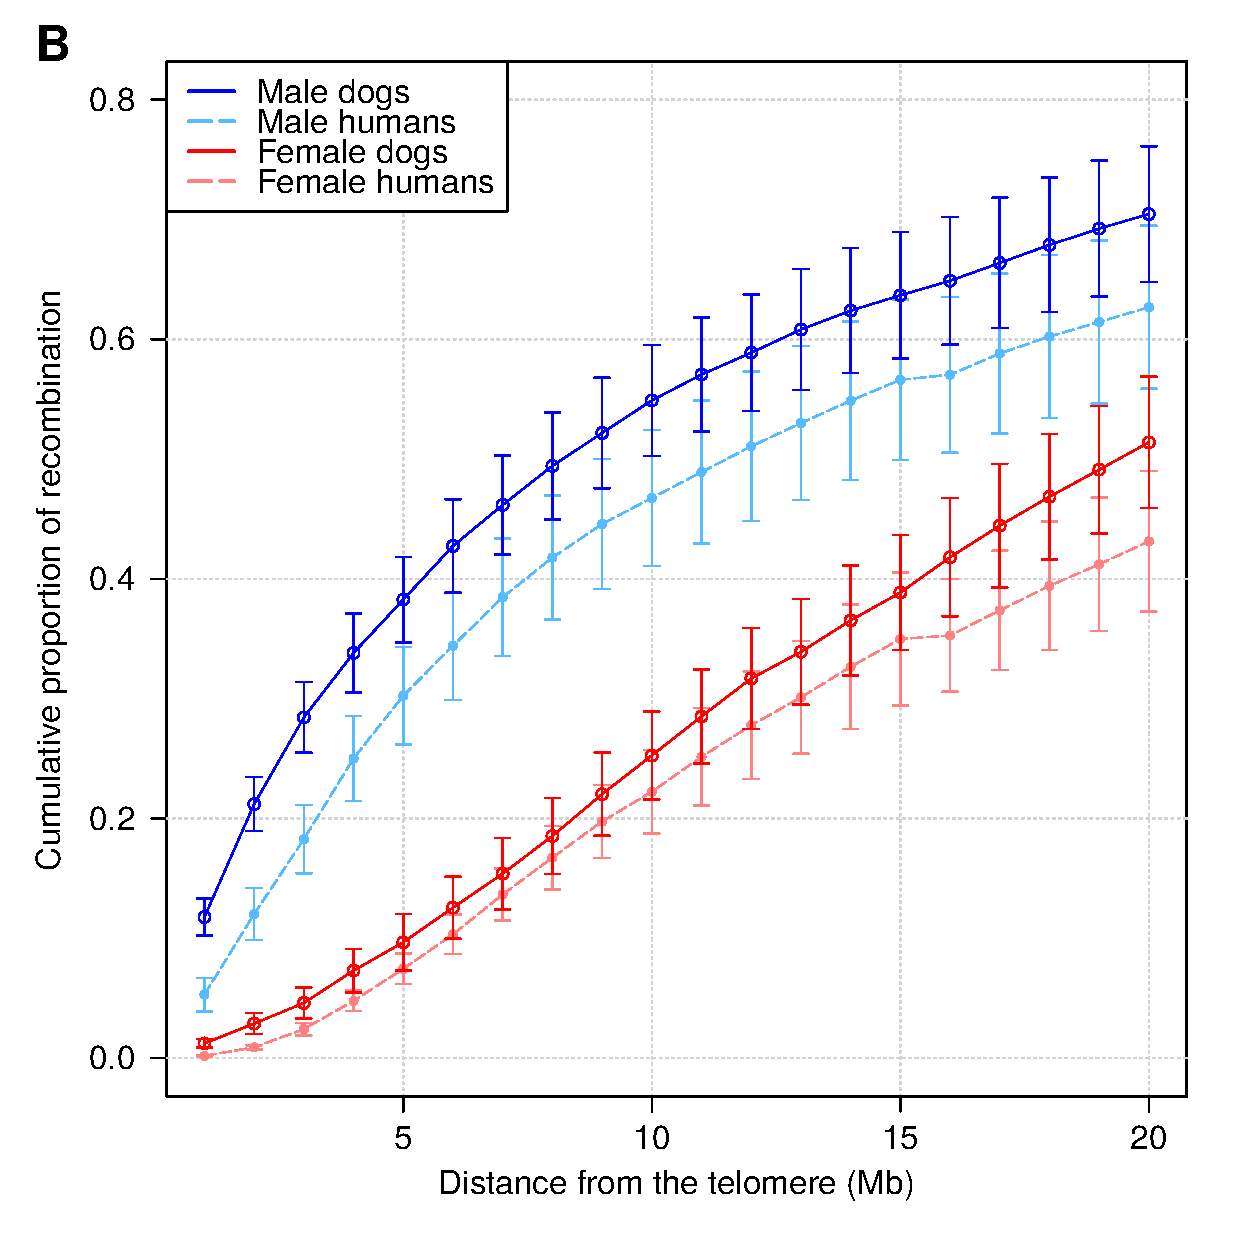
\includegraphics[width=0.5\textwidth]{dogPed/figs/propTelRecomb_Mb}
    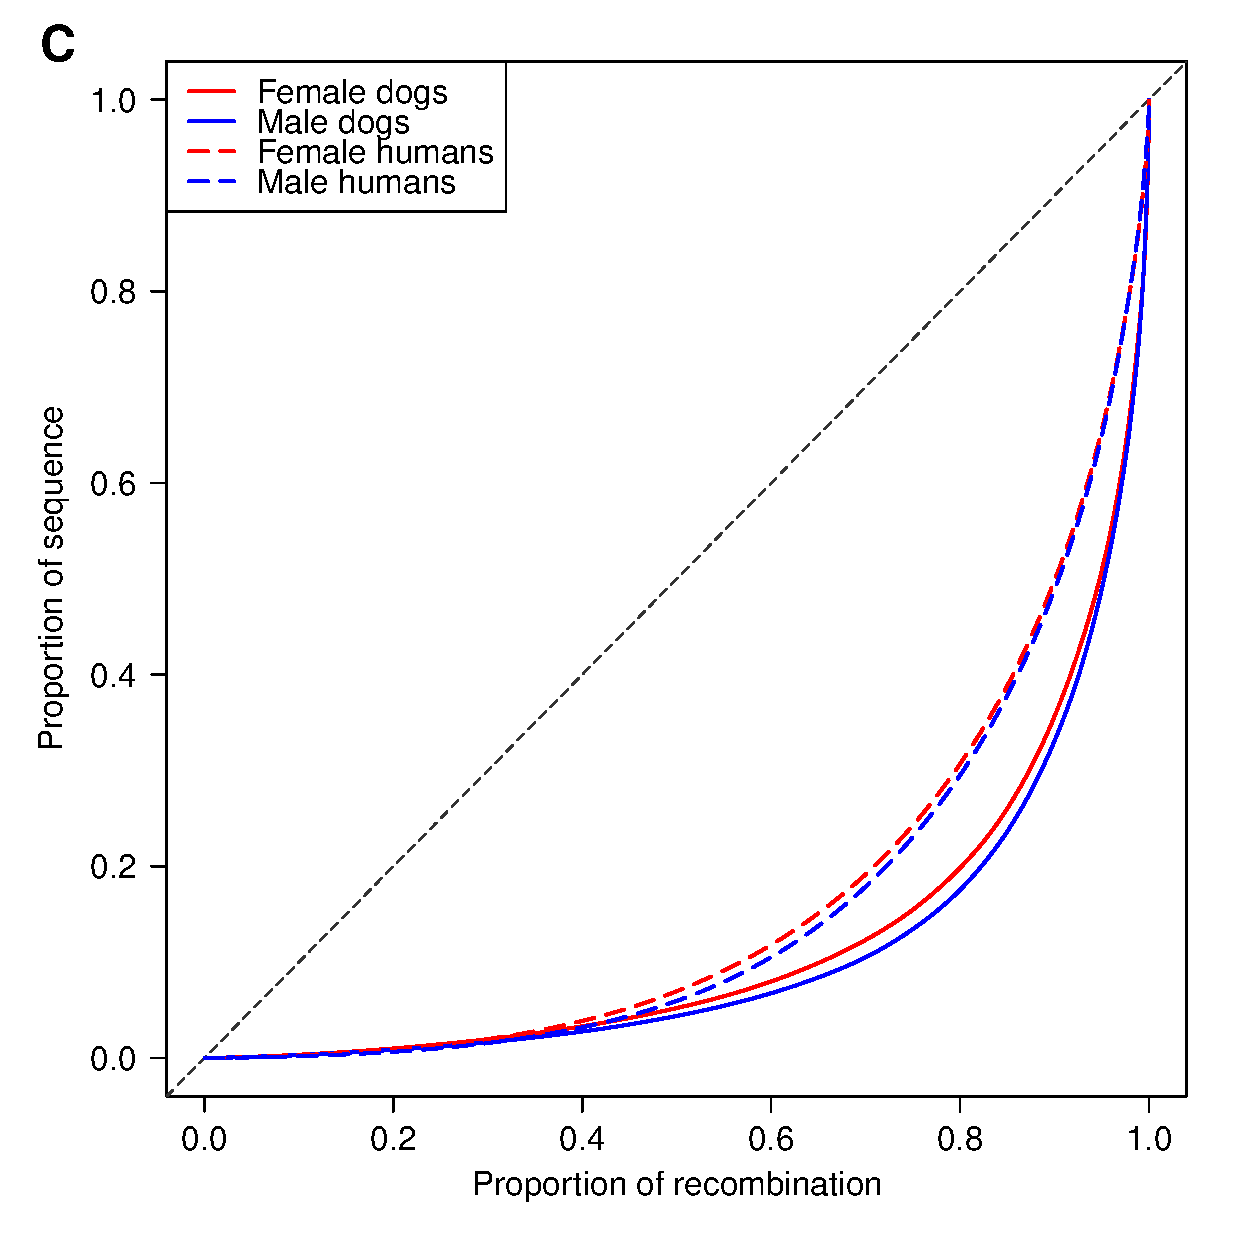
\includegraphics[width=0.5\textwidth]{dogPed/figs/8020plot_human-dog}
    \vspace{-15pt}
    \caption{The distribution of recombination across the genome.
        (A) Broad scale recombination rates differ between males and females.  Rates were smoothed at the 5 Mb scale. Chromosomes 27 and 32 are likely reversed in the canFam3.1 genome build, and are shown here with their physical coordinates reversed.
        %(B) The proportion of recombination occurring in subtelomeric regions of the genome as a function of chromosome arm length.
        (B) The proportion of recombination as a function of the distance from the telomeric end of each chromosome arm. Error bars represent a 95\% confidence interval.
        (C) Proportion of recombination occupying various fractions of the sequence. The human data were thinned to match the SNP density and meiosis count of the dog dataset.
        For all panels, males and females are shown in shades of blue and red, respectively. Human data in panels B and C is shown in dashed lines.
    \label{fig:distrRecomb}}
\end{figure}
\clearpage}


%, indicating that male recombination is more concentrated at the telomere.
% We estimate the amount of recombination occurring towards the telomeric ends of each chromosome, taking the most distal 15\% of each chromosome arm by physical distance (Figure \ref{fig:distrRecomb}B).
% Male dogs have a higher proportion of recombination, 45.9\%, occurring in this telomeric portion, compared to only 13.4\% in females.
% A similar pattern is observed in humans (males 39.9\%, females 16.3\%).
% %shows a significantly higher proportion of recombination in the telomeres of male dogs ($p=0.007$) but no difference between species for females ($p=0.257$).
% %Fitting a linear model with terms for species 
% Using linear  regression,
% chromosome arm length is a significant predictor of the proportion of telomeric recombination in females ($p=1.15 \times 10^{-11}$) but not males ($p=0.118$).
% Using species as a predictor, dogs and humans have indistinguishable trends for females ($p=0.257$), 
% while in males, dogs and humans are significantly different ($p=0.007$), possibly due to increased variance in the dog data. 
% %%%
% Furthermore, adding an interaction term between arm length and species shows no significant differences in the slopes of the regression lines between species for either sex (male $p=0.71$, female $p=0.08$).
% %With the exception of chromosomes 16, 17, and 32, male recombination is concentrated at the telomeres.
% %Humans show a similar overall pattern, with males having a higher proportion of recombination occurring towards telomeres (30.7\% in males, 5.4\% in females).
% We conclude that, at a broad scale, telomeric recombination in dogs is similar to that of humans and appears to be dependent on chromosome arm size in females.

%%% Uniformity of recomb distrib in dogs
Previous observations using LD recombination maps have raised the possibility that dog recombination may be more uniform in distribution throughout the genome than in humans due to the loss of \textit{PRDM9}\cite{Axelsson2012,Auton2013}.
% When estimating the proportion of recombination that occupies a given amount of sequence, 
% the majority of dog recombination (80\%) was found to occur in 30-46\% of the sequence\cite{Axelsson2012,Auton2013},
% while human recombination was concentrated into less than 20\% of sequence\cite{Myers2005,1000G2010}.
However, estimates from LD can be confounded by differences in the effective population size, which complicate such comparisons.
Pedigree-based studies should not be subject to the same confounding issues, and
to investigate this further, we examined the concentration of recombination rates across the genome using our pedigree maps, and compared this to human pedigree data\cite{Campbell2015}.
This analysis is sensitive to the marker coverage and crossover resolution, so the human genetic maps have been reduced in resolution to match that of the dog data (see Methods, Figures \ref{fig:8020supp}A and C).
We found that 80\% of recombination occurred in a smaller proportion of the dog genome (17.5\% male, 19.8\% female, Figure \ref{fig:distrRecomb}C) than previously reported in LD-based estimates.
In contrast to the LD-based findings, dog recombination is actually less uniform than in the human thinned data,
in which males have 29.5\%, and females 30.7\% of their sequence containing the majority (80\%) of recombination.
In addition, males of both species have more focused recombination when compared to females.
To address the possibility that differences in genome architecture or recombination rate distribution could account for these observations, we excluded telomeric regions from the analysis, and matched dog chromosomes with similarly sized human chromosome arms (Figures \ref{fig:8020supp}B and D), with similar results.
Therefore, it appears that crossovers are more concentrated within a smaller proportion of the dog genome than in humans, and that this effect is more pronounced in males of both species.

\paragraph{Recombination around genomic features.}

Starting from the observation that recombination is targeted to CpG islands concentrated at gene promoter regions\cite{Auton2013}, we looked for these effects in our data, and to what extent they are sex specific.
We found that recombination rates were elevated around the TSS, both in the sex averaged and male maps, but no peak was discernible in females (Table \ref{tab:recRates}, Figure \ref{fig:genomicFeatures}A).
Additionally, male recombination rate in the surrounding regions was higher than females, despite a lower genome wide recombination rate.
This observation that can be partially explained by a modest enrichment in the number of genes (31\%) occurring in the telomeric 25\% of each chromosome where male recombination is more frequent.
However, while the male background rate is higher in telomeric regions, males exhibited a peak at the TSS even in non-telomeric regions (Figure \ref{fig:TSScpgSplit}A and B).

Both male and female recombination estimates showed elevated recombination surrounding CpG islands (Table \ref{tab:recRates}, Figure \ref{fig:genomicFeatures}B).
The peak in male dogs was higher than females by 0.98 cM/Mb, with a high background rate in the surrounding sequence, which could be explained by
clustering of CpGs, as well as an enrichment of CpG islands in telomeric, male driven recombination regions (42\% in 25\% of sequence, Figure \ref{fig:TSScpgSplit}C and D).
After thinning CpG islands to a uniform density throughout the genome, the male and female background rates were more comparable, but the male peak remains higher, suggesting that recombination around CpG islands is dominated by males (Figure \ref{fig:cpgThinned}).
We also examined recombination rates around H3K4 trimethylation marks found via ChIPseq on dog spermatocytes\cite{Auton2013}.
As previously reported, the presence of these marks associated with elevated recombination rates, however this association can be explained by the proximity of CpG islands to H3K4me3 marks (Figure \ref{fig:H3K4panel}), and we saw no differences between males and females.

% \paragraph{Hotspot usage}

\paragraph{Crossover interference.}
Crossover interference, a phenomenon that affects the physical spacing between pairs of crossover events occurring during the same meiosis, acts in various species, including humans\cite{Campbell2015,Broman2000,Housworth2003}, mice\cite{Broman2002}, and cattle\cite{Sandor2012}.
To learn more about interference in dogs, we examined the distribution of inter-crossover distances in our dataset.
We fit two models of crossover interference, the gamma model\cite{Broman2000}, and the gamma-escape model\cite{Housworth2003} (also known as the Housworth-Stahl model).
The gamma-escape model is a mixture model that builds upon the gamma model, adding a subset of events that escape interference.

The no-interference model ($\nu=1$), had a poor fit, with a lack of double crossovers in close proximity, indicating that positive crossover interference must be acting to some degree in dogs.
When fitting the simple gamma model, estimates of interference strength in male and female dogs overlapped with each other. % ($\nu_{female}=5.22$, $\nu_{male}=3.73$).
These estimates are comparable to a cytological study in dogs measuring the distance between MLH1 foci, which mark crossovers ($\nu$=6.1)\cite{Basheva2008}.
Comparing to humans, female dogs have a stronger strength of interference than human females, while the estimates for males of both species overlap (Figure \ref{fig:cointGenome}A, Table \ref{tab:cointParams}).
%The interference strength estimates in the gamma model are roughly comparable to those observed in humans

\afterpage{
\begin{figure}[p]
    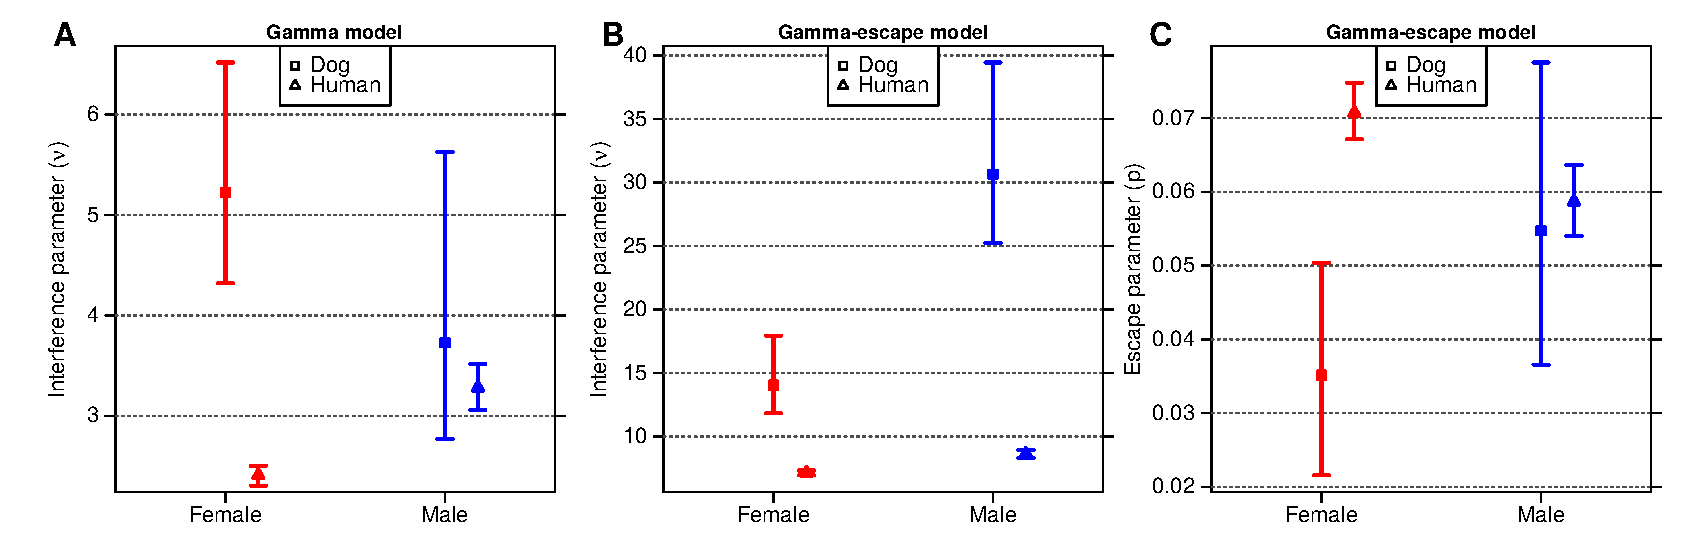
\includegraphics[width=\textwidth]{dogPed/figs/interferenceParameters_genome}
    \vspace{-20pt}
    \caption{Estimates of crossover interference parameters in the dog genome using the simple gamma model (A) and Housworth-Stahl gamma-escape model (B and C).
       Panels A and B show the interference strength parameter, $\nu$, for each model, while
       the right panel (C) shows the escape parameter, $p$, the proportion of events that escape interference.
       Males are shown in blue and females in red, while estimates for dogs are shown in boxes, and humans in triangles.
       The error bars represent a 95\% confidence interval estimated from 1000 bootstrap iterations. \label{fig:cointGenome}}
\end{figure}
\clearpage}

In the interference-escape model,
estimates of the strength of interference across the dog genome are higher in males than in females ($\nu_{female}=14.05$, $\nu_{male}=30.64$).
This trend is similar to that seen in humans, with stronger crossover interference in males, however the parameter estimates are higher by a factor of 2 in females, and more than 3 in males ($\nu_{female}=7.19$, $\nu_{male}=8.93$ in humans, Figure \ref{fig:cointGenome}B).
In contrast, male dogs have a similar proportion of escaping events to humans (5.5\% vs 5.9\%), while
female dogs have fewer events (3.5\%) escaping than human females (7.1\%, Figure \ref{fig:cointGenome}C).
We found support for both models of interference in the dog dataset, however
we used BIC to make a formal comparison of the goodness of fit for each model.
We found that in both sexes the gamma-escape model is preferred over the simple gamma model (Table \ref{tab:cointParams}), in agreement with previous findings supporting a two-pathway model of crossover interference in humans\cite{Housworth2003,Campbell2015}.


\afterpage{
\begin{table}[p] \centering
    \small
    \begin{tabular}{|c|c|c|c|c|c|} \hline 
            & \multicolumn{2}{c|}{Gamma model} & \multicolumn{3}{c|}{Gamma-escape model} \\ \hline
            & $\nu$ (95\% CI) & BIC & $\nu$ (95\% CI) & $p$ (95\% CI) & BIC \\ \hline
        Male dogs   & 3.73 (2.77-5.63) & 6617.1 & 14.05 (11.82-17.95) & 0.055 (0.037-0.078) & 6174.6 \\
        Female dogs & 5.22 (4.32-6.52) & 7580.9 & 30.64 (25.23-39.44) & 0.035 (0.022-0.050) & 7274.0 \\
        \hline
        Male humans   & 3.28 (3.06-3.51) & 99043.7  & 8.63 (8.29-8.96) & 0.059 (0.054-0.064) & 93205.3 \\
        Female humans & 2.41 (2.31-2.50) & 168775.7 & 7.13 (6.95-7.33) & 0.071 (0.067-0.075) & 156793.4 \\
    \hline \end{tabular}
    \caption{Autosomal crossover interference.  Parameter estimates are shown for both gamma and gamma-escape models for combined autosomes in dogs and humans.  Numbers in parentheses represent 95\% confidence intervals. BIC, Bayesian Information Criterion. \label{tab:cointParams}}
\end{table}
\clearpage}

To test if this difference reflects a change in interference parameters with parental age, as is observed in humans\cite{Campbell2015},
%To see if this difference is due to an increase in escape from crossover interference with age, as observed in humans,
we divided our dataset by age into 7 approximately equal sized bins.
No differences were observed for crossover parameters for either model in any of the age groups (Figure \ref{fig:cointGenomeAge}).
However, we should note that bootstrapped estimates produce large error bars and there is likely insufficient power to adequately detect any age differences in this dataset.

When reducing the resolution of the human dataset (see Methods), we found that the parameter estimates were largely unchanged compared to those of the full resolution data, although with wider confidence intervals (Figure \ref{fig:cointGenomeThin}).
This provides confidence that parameter estimation using these models is robust to crossover interval size resolution and dataset power,
and that the parameters estimated from our dog data are likely to accurately reflect those of this dataset.

%%%%%%%%%%%%%%%%%%%%%%%%%%%%%%%%%%%%%%%%
%%%%%%%%%%%%%%%%%%%%%%%%%%%%%%%%%%%%%%%%
\section{Discussion}
%%%%%%%%%%%%%%%%%%%%%%%%%%%%%%%%%%%%%%%%
%%%%%%%%%%%%%%%%%%%%%%%%%%%%%%%%%%%%%%%%

Since the discovery of PRDM9 and its importance to recombination, questions about its full role have persisted.
While \textit{PRDM9} is under selection across a variety of species\cite{Oliver2009}, a notable subset are missing a functional version of this protein, raising questions regarding the landscape of recombination in these species.
%including canids, in which an apparently once functional version was rendered a pseudogene via mutation at some point in their evolutionary past.
Our pedigree study adds to existing work and provides insight into recombination in the absence of \textit{PRDM9}.
On a broad scale, our results are in agreement with those from previous studies, demonstrating that dog recombination is similar to other mammals, indicating that the presence or lack of \textit{PRDM9} does not change broad scale patterns of crossover placement.
In particular, a majority of crossing over occurs in telomeric regions in males, while female crossing over is both more frequent and more spread out.

We report a ratio of female to male map lengths of 1.19, equivalent to previous estimates from \citet{Wong2010}.
This groups domestic dogs with a large collection of species that exhibit sexual dimorphism in recombination in which the female has a higher rate of crossing over, including humans\cite{Campbell2015} and mice\cite{Cox2009}.
%This effect is more extreme in humans, with a ratio of 1.56\cite{Campbell2015}
In contrast, cattle are one of the few species that have the opposite trend, with a recent study in domestic cattle estimating the male map length to be 10\% longer than females\cite{Ma2015}.
An interesting suggestion from this study was that the overall recombination rate in males may have been affected by artificial selection pressure.
Because artificial selection is more frequently focused on males, this can result in an increase in recombination if selection acts positively on recombination rate.
If true, it is not implausible that this selective pressure could have altered recombination in dogs during their domestication as well, something that could be revealed through a comparison to wolves, the closest ancestor to the modern domestic dog.
 
Initial estimates using LD maps in dogs indicated that 80\% of all recombination falls into a fairly large (30-46\%) amount of sequence\cite{Axelsson2012,Auton2013}, markedly more spread out than the $<$20\% figure seen in human LD maps\cite{hapmap2007}.
This supports the idea that PRDM9 acts to funnel recombination into hotspots in humans, and supports the hypothesis that dog recombination, lacking this hotspot specifying protein, is more uniform across the genome.
While further investigation is necessary,
our findings here, using pedigree data, suggest that dog recombination may actually be less uniform than humans.
Furthermore, in both species, males appear slightly more focused than females.  
This effect in humans could potentially be explained by a higher male hotspot usage\cite{Campbell2015}.
In dogs, this could be due to higher male rates around gene promoter regions and CpG islands that are concentrated towards the telomeres.
This concentration of recombination at functional genomic elements is not unique to dogs, but appears to be shared among a number of species lacking \textit{PRDM9}, including \textit{PRDM9} knockout mice\cite{Brick2012},
Arabidopsis, yeast\cite{Lam2015}, and birds\cite{Singhal2015}.

The concentration of recombination at these functional elements
supports a working model for \textit{PRDM9}-absent species, in which recombination occurs preferentially in regions of open chromatin.
Another implication is that recombination hotspots in dogs and other \textit{PRDM9}-absent species may be stable in evolutionary time, in contrast to current evidence against hotspot sharing in \textit{PRDM9} dependent species.
Since dog hotspots lack a strong motif that is likely to be targeted by a trans acting factor such as PRDM9\cite{Axelsson2012,Auton2013}, they are not likely to be subject to the hotspot paradox that acts to continually erode the binding capacity of hotspots, even as they are actively being used for recombination\cite{Myers2010}.
Evidence for hotspot stability has been found in two finch species, which share recombination hotspots that appear to be separated by tens of millions of years\cite{Singhal2015}, as well as four yeast species sharing hotspots over 15 million years of evolution\cite{Lam2015}.


%hotspots, evolutionary stability of hotspots in dogs.
%%% %%% discussion of finch / yeast hotspot science papers here:

%A recent study of methylation and substitution rates in dogs suggests that 
%recombination is high in promoter associated hotspots,
%in which CpG islands have low germline methylation, and therefore low mutability.
%By contrast, the recombination rate near highly-mutable methylated CpG islands away from promoters is lower, the GC content having increased as a result of biased gene conversion (BGC), the preferential transfer of G/C alleles over A/T alleles that occurs as a byproduct of mismatch repair during recombination\cite{Berglund2015}.
%and is therefore tied to a lack of germline methylation in these regions.



The distribution of inter-crossover distances in dogs supports the existence of positive crossover interference in the dog genome.
Estimates of interference strength in the simple gamma model are roughly in line with those in humans.
However, our results favor the gamma-escape model, supporting the idea that two separate pathways contribute to recombination in dogs.
%This implies that neither pathway is wholly dependent on PRDM9, though
In this model, dog interference appears to be 2-3 times stronger than in humans, with a similar proportion of escaping events.
% evidence for positive crossover interference implies PRDM9 is not involved with interference.
%%%%%%%
Interestingly, while an increase in interference escape with age has been observed in human females\cite{Campbell2015}, no such age effect was observed in dogs.
Accepting that our canine sample size would limit our ability to detect such effects, another
potential explanation is that, in contrast to humans, 
% there is no evidence that the timing of meiotic arrest is the same in female dogs.
% is that there is an increase in escaping crossovers forming during the extended prenatal meiotic arrest period.
the timing of meiotic events in dogs is substantially different.
Recombination in human females begins and enters a potentially lengthy meiotic arrest prenatally, resuming just prior to ovulation.
In contrast, meiosis in female dogs begins later, in the neonatal period. %, and enters a similarly timed arrest (prior to completion of prophase I),
While recombination is complete prior to ovulation in humans, dogs ovulate immature oocytes, after which meiosis must complete before the oocyte becomes fertile, around 48 hours after ovulation\cite{Freixa1987,Chastant-Maillard2011}.

% While recombination in human females begins and enters a potentially lengthy meiotic arrest prenatally, in female dogs meiosis I begins in the neonatal period, arresting  before the completion of prophase I.
% While recombination is complete prior to ovulation in humans, dogs ovulate immature oocytes, after which and meiosis must complete before the oocyte becomes fertile\cite{Freixa1987,Chastant-Maillard2011}.
%However it appears that a similarly timed meiotic arrest is absent in female dogs;
%Instead, prophase of meiosis I begins in the neonatal period, and arrests before completion of prophase I.
%Immature oocytes are then ovulated, after which meiosis must complete before the oocyte becomes fertile\cite{Freixa1987,Chastant-Maillard2011}.
%%%%%%

Overall, these results add to a growing body of research in non-human recombination genetics, 
and provide a step towards answering many open questions in canine recombination.
Further work is needed on larger and more diverse pedigrees, both in domestic dogs and other members of the Canidae family, including wolves, in order to form a more complete picture of recombination in this family.

%, primarily the effect of the loss of PRDM9 on crossover placement.
%However, we cannot exclude the possibility that our dataset, comprised of a relatively small number of inbred dogs of two breeds, has limited our power to adequately detect some of the effects presented here.
%Nevertheless, we provide here an updated high resolution dog genetic map that can be used to provide further insight into dog recombination, as well as to inform other aspects of canine genomics.


% hotspots
%Despite the absence of PRDM9 in the dog genome, crossovers still cluster into hotspot-like regions, and these tend to be CpG rich regions that occur near gene promoters\cite{Axelsson2012,Auton2013}.
%This pattern is similar to that in other species lacking PRDM9, including birds\cite{Singhal2015}, yeast\cite{Lam2015}, and knockout mice\cite{Brick2012}.
%, in which recombination targets H3K4me3 marks present on gene promoters\cite{Brick2012}.

\section{Acknowledgments}
We thank Yu Kong and Anthony Marcketta for their helpful discussions and assistance in the analysis of this data.
C.L.C.\ was supported by the Training Program in Cellular and Molecular Biology and Genetics, T32 GM007491.
C.B. was supported by a postdoctoral fellowship from the Fonds de la recherche en sant\'{e} du Qu\'{e}bec (FRQS).
Data in this paper are from a thesis to be submitted in partial fulfillment of the requirements for the Degree of Doctor of Philosophy in the Graduate Division of Medical Sciences, Albert Einstein College of Medicine, Yeshiva University.

%\section{Author Contributions}
%[To do.]


%%%%%%%%%%%%%%%%%%%%%%%%%%%%%%%%%%%%%%%%
%%%%%%%%%%%%%%%%%%%%%%%%%%%%%%%%%%%%%%%%
\clearpage
\renewcommand{\bibname}{References}
\bibliographystyle{ccampbell_thesis}
\begingroup
    \setlength{\bibsep}{10pt}
    \linespread{1}\selectfont
    \bibliography{dogPed/dogPed}
\endgroup
%%%%%%%%%%%%%%%%%%%%%%%%%%%%%%%%%%%%%%%%
%%%%%%%%%%%%%%%%%%%%%%%%%%%%%%%%%%%%%%%%

\clearpage
%%%%%%%%%%%%%%%%%%%%%%%%%%%%%%
%%%%%%%%%%%%%%%%%%%%%%%%%%%%%%
% Supplement
%%%%%%%%%%%%%%%%%%%%%%%%%%%%%%
%%%%%%%%%%%%%%%%%%%%%%%%%%%%%%
\beginsupplement
\section{Supplementary Information}

\begin{table}[h] \centering
    \begin{tabular}{|c|c|c|c|c|} 
        \hline Chromosome & Start & End & Size & \# variants \\ \hline
        6 & 44745965 & 47085070 & 2339105 & 182 \\
        16 & 53878711 & 56703603 & 2824892 & 221 \\
        19 & 20011075 & 20320803 & 309728 & 24 \\
        32 & 38654394 & 38810281 & 155887 & 8 \\
        \hline &&   \textbf{Total}   &   \textbf{5629612}    &   \textbf{435} \\
    \hline \end{tabular}
    \captionTitle{\textbf{Regions removed from the dataset.}}{\label{tab:badregions}}
\end{table}

\begin{table}[p] \centering
    \scriptsize
    \begin{tabular}{|c|p{1.3cm}|p{1.3cm}|p{1.2cm}|p{0.8cm}|p{0.8cm}|p{0.8cm}|p{0.8cm}|p{0.8cm}|p{0.8cm}|p{0.8cm}|}
        \hline CFA & Physical (bp) & First position (bp) & Last position (bp) & Female (cM) & Mean female rate (cM/Mb) & Male (cM) & Mean male rate (cM/Mb) & Sex avg.\ (cM) & Sex avg.\ rate (cM/Mb) & No. markers \\ \hline
1 & 122,678,785 & 4,283,592 & 122,309,715 & 95.54 & 0.78 & 85.17 & 0.69 & 90.12 & 0.73 & 8284 \\
2 & 85,426,708 & 3,621,442 & 85,062,551 & 78.36 & 0.92 & 64.77 & 0.76 & 71.66 & 0.84 & 5550 \\
3 & 91,889,043 & 5,604,604 & 91,556,345 & 75.63 & 0.82 & 62.64 & 0.68 & 68.77 & 0.75 & 6681 \\
4 & 88,276,631 & 5,840,941 & 87,934,673 & 76.46 & 0.87 & 55.85 & 0.63 & 66.10 & 0.75 & 6231 \\
5 & 88,915,250 & 1,243,143 & 88,673,195 & 95.67 & 1.08 & 68.00 & 0.76 & 81.70 & 0.92 & 6432 \\
6 & 77,573,801 & 455,434 & 77,489,595 & 67.30 & 0.87 & 59.17 & 0.76 & 63.11 & 0.81 & 5320 \\
7 & 80,974,532 & 180,153 & 80,809,723 & 70.31 & 0.87 & 47.59 & 0.59 & 58.81 & 0.73 & 5778 \\
8 & 74,330,416 & 2,763,496 & 72,510,424 & 60.10 & 0.81 & 57.07 & 0.77 & 57.83 & 0.78 & 4846 \\
9 & 61,074,082 & 876,259 & 60,812,630 & 62.66 & 1.03 & 50.65 & 0.83 & 55.67 & 0.91 & 4293 \\
10 & 69,331,447 & 2,125,046 & 69,293,175 & 66.85 & 0.96 & 55.26 & 0.80 & 61.17 & 0.88 & 4573 \\
11 & 74,389,097 & 4,087,888 & 74,253,347 & 58.71 & 0.79 & 48.36 & 0.65 & 53.60 & 0.72 & 4557 \\
12 & 72,498,081 & 82,400 & 72,115,946 & 61.01 & 0.84 & 52.90 & 0.73 & 55.91 & 0.77 & 5364 \\
13 & 63,241,923 & 4,067,434 & 62,932,928 & 54.05 & 0.85 & 45.71 & 0.72 & 49.52 & 0.78 & 4749 \\
14 & 60,966,679 & 7,309,849 & 60,600,364 & 51.49 & 0.84 & 45.22 & 0.74 & 48.11 & 0.79 & 4153 \\
15 & 64,190,966 & 4,913,124 & 64,007,939 & 48.69 & 0.76 & 44.57 & 0.69 & 46.43 & 0.72 & 4372 \\
16 & 59,632,846 & 6,692,748 & 58,967,916 & 52.23 & 0.88 & 37.86 & 0.63 & 45.03 & 0.76 & 3829 \\
17 & 64,289,059 & 5,285,642 & 63,501,532 & 63.44 & 0.99 & 50.07 & 0.78 & 56.58 & 0.88 & 4731 \\
18 & 55,844,845 & 3,203,856 & 55,355,125 & 55.33 & 0.99 & 52.01 & 0.93 & 53.71 & 0.96 & 4014 \\
19 & 53,741,614 & 3,189,264 & 53,349,320 & 53.22 & 0.99 & 49.99 & 0.93 & 52.29 & 0.97 & 3733 \\
20 & 58,134,056 & 4,356,904 & 58,000,062 & 52.64 & 0.91 & 55.38 & 0.95 & 53.59 & 0.92 & 4140 \\
21 & 50,858,623 & 4,450,666 & 50,719,350 & 51.66 & 1.02 & 44.16 & 0.87 & 47.84 & 0.94 & 3706 \\
22 & 61,439,934 & 2,513,263 & 61,217,407 & 52.21 & 0.85 & 49.67 & 0.81 & 50.57 & 0.82 & 4422 \\
23 & 52,294,480 & 1,203,392 & 52,291,577 & 49.31 & 0.94 & 44.47 & 0.85 & 46.63 & 0.89 & 3928 \\
24 & 47,698,779 & 1,029,209 & 47,233,919 & 49.71 & 1.04 & 53.74 & 1.13 & 51.50 & 1.08 & 3625 \\
25 & 51,628,933 & 6,038,820 & 51,469,123 & 56.49 & 1.09 & 48.57 & 0.94 & 52.44 & 1.02 & 3922 \\
26 & 38,964,690 & 2,407,850 & 38,657,286 & 46.66 & 1.20 & 41.16 & 1.06 & 43.81 & 1.12 & 2853 \\
27 & 45,876,710 & 444,525 & 42,191,669 & 48.31 & 1.05 & 48.70 & 1.06 & 47.01 & 1.02 & 3354 \\
28 & 41,182,112 & 4,526,049 & 40,963,512 & 51.11 & 1.24 & 39.62 & 0.96 & 45.41 & 1.10 & 3074 \\
29 & 41,845,238 & 913,671 & 41,543,120 & 49.96 & 1.19 & 42.06 & 1.01 & 44.75 & 1.07 & 3017 \\
30 & 40,214,260 & 5,433,983 & 39,826,282 & 43.89 & 1.09 & 37.30 & 0.93 & 40.20 & 1.00 & 2942 \\
31 & 39,895,921 & 580,882 & 39,466,279 & 51.82 & 1.30 & 38.07 & 0.95 & 44.32 & 1.11 & 2855 \\
32 & 38,810,281 & 114,049 & 37,999,255 & 46.13 & 1.19 & 41.68 & 1.07 & 43.78 & 1.13 & 2746 \\
33 & 31,377,067 & 447,033 & 30,994,965 & 45.46 & 1.45 & 36.01 & 1.15 & 40.75 & 1.30 & 2320 \\
34 & 42,124,431 & 624,977 & 41,979,553 & 48.69 & 1.16 & 38.71 & 0.92 & 43.36 & 1.03 & 3239 \\
35 & 26,524,999 & 1,164,664 & 26,257,078 & 41.87 & 1.58 & 30.59 & 1.15 & 35.88 & 1.35 & 2171 \\
36 & 30,810,995 & 251,708 & 30,523,428 & 41.77 & 1.36 & 29.61 & 0.96 & 35.95 & 1.17 & 2286 \\
37 & 30,902,991 & 1,364,851 & 30,583,437 & 45.59 & 1.48 & 36.18 & 1.17 & 40.42 & 1.31 & 2333 \\
38 & 23,914,537 & 246,006 & 23,695,770 & 41.67 & 1.74 & 27.38 & 1.15 & 33.68 & 1.41 & 1895 \\
 \hline &  &  & \textbf{Total} & 2161.99 & 0.98 & 1815.91 & 0.82 & 1978.01 & 0.90 & 156,318 \\
\hline \end{tabular}
\captionTitle{\textbf{Physical and genetic chromosome lengths.}}{ \label{tab:mapLengths}}
\end{table}

\begin{table}[p] \centering
    \begin{tabular}{|c|c|c|c|c|} \hline 
        & Size (kb) & Male rate & Female rate & Difference (male - female) \\ \hline
        TSS upstream & 400 & 1.01 & 0.92 & 0.09 \\
        TSS & 50 & 1.12 & 0.92 & 0.20 \\
        TSS downstream & 400 & 1.03 & 0.94 & 0.09 \\
        \hline
        CpG upstream & 400 & 1.84 & 0.95 & 0.89 \\
        CpG island & 50 & 2.09 & 1.11 & 0.98 \\
        CpG downstream & 400 & 1.75 & 0.97 & 0.78 \\
    \hline \end{tabular}
    \captionTitle{\textbf{Recombination rate around TSS and CpG islands.}}{ Recombination rates are given in cM/Mb and were estimated in 10kb bins, and averaged over the indicated window.
        Rates surrounding CpG islands represent a 50kb window centered around the CpG island, while rates for the TSS are given as a 50kb bin ending at the TSS, capturing the elevated rate immediately upstream.
    \label{tab:recRates}}
\end{table}

\clearpage

\begin{figure}[p]
    \centering
    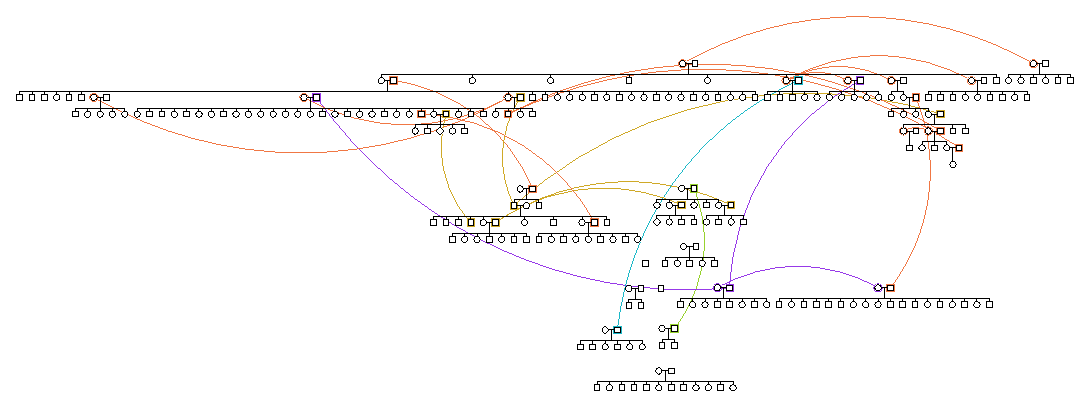
\includegraphics[width=\textwidth]{dogPed/suppfigs/dogPedigreePlot}
    \vspace{-5pt}
    \captionTitle{\textbf{Structure of the dog pedigree.}}{
        Males are represented by squares, females by circles.
        Colored lines indicate individuals repeated on the plot, that are involved in more than one mating pair.
    \label{fig:pedigree}}
\end{figure}

\begin{figure}[p]
    \centering
    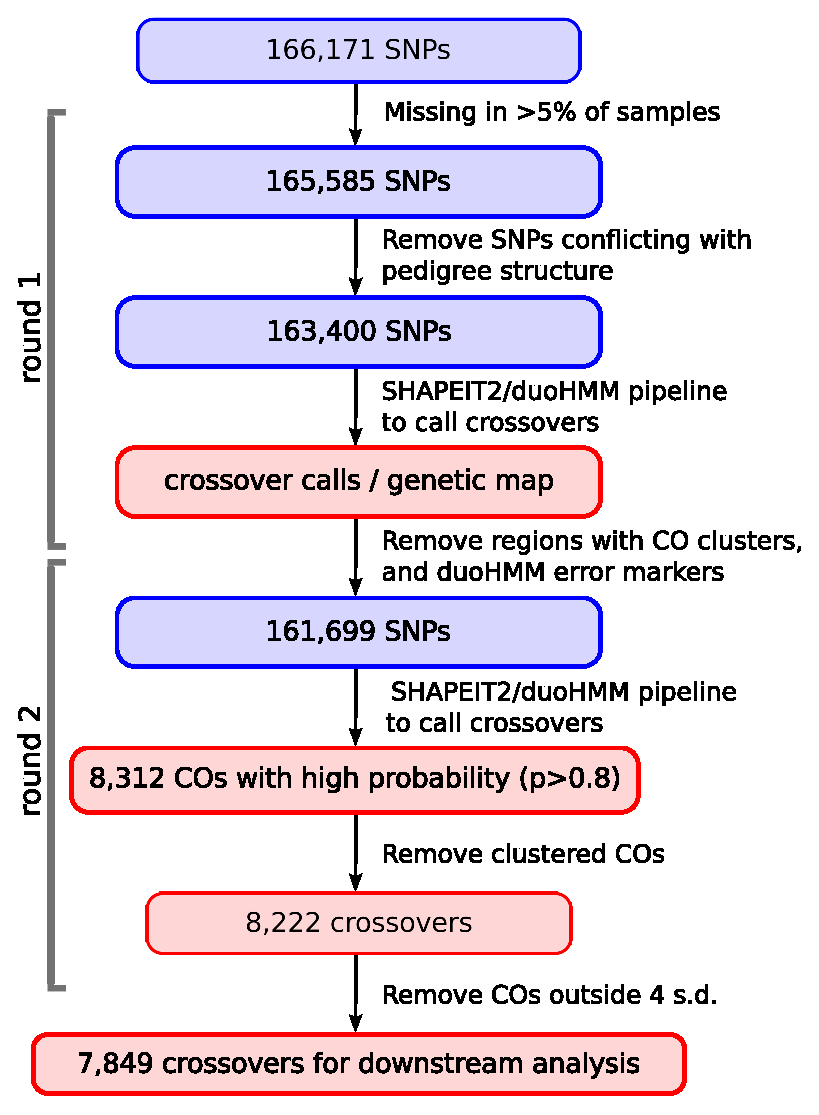
\includegraphics[height=0.6\textheight]{dogPed/suppfigs/pipeline}
    \vspace{-5pt}
    \captionTitle{\textbf{Overview of the analysis pipeline.}}{
        CO, crossovers; s.d., standard deviation.
    \label{fig:pipeline}}
\end{figure}

\begin{figure}[p]
    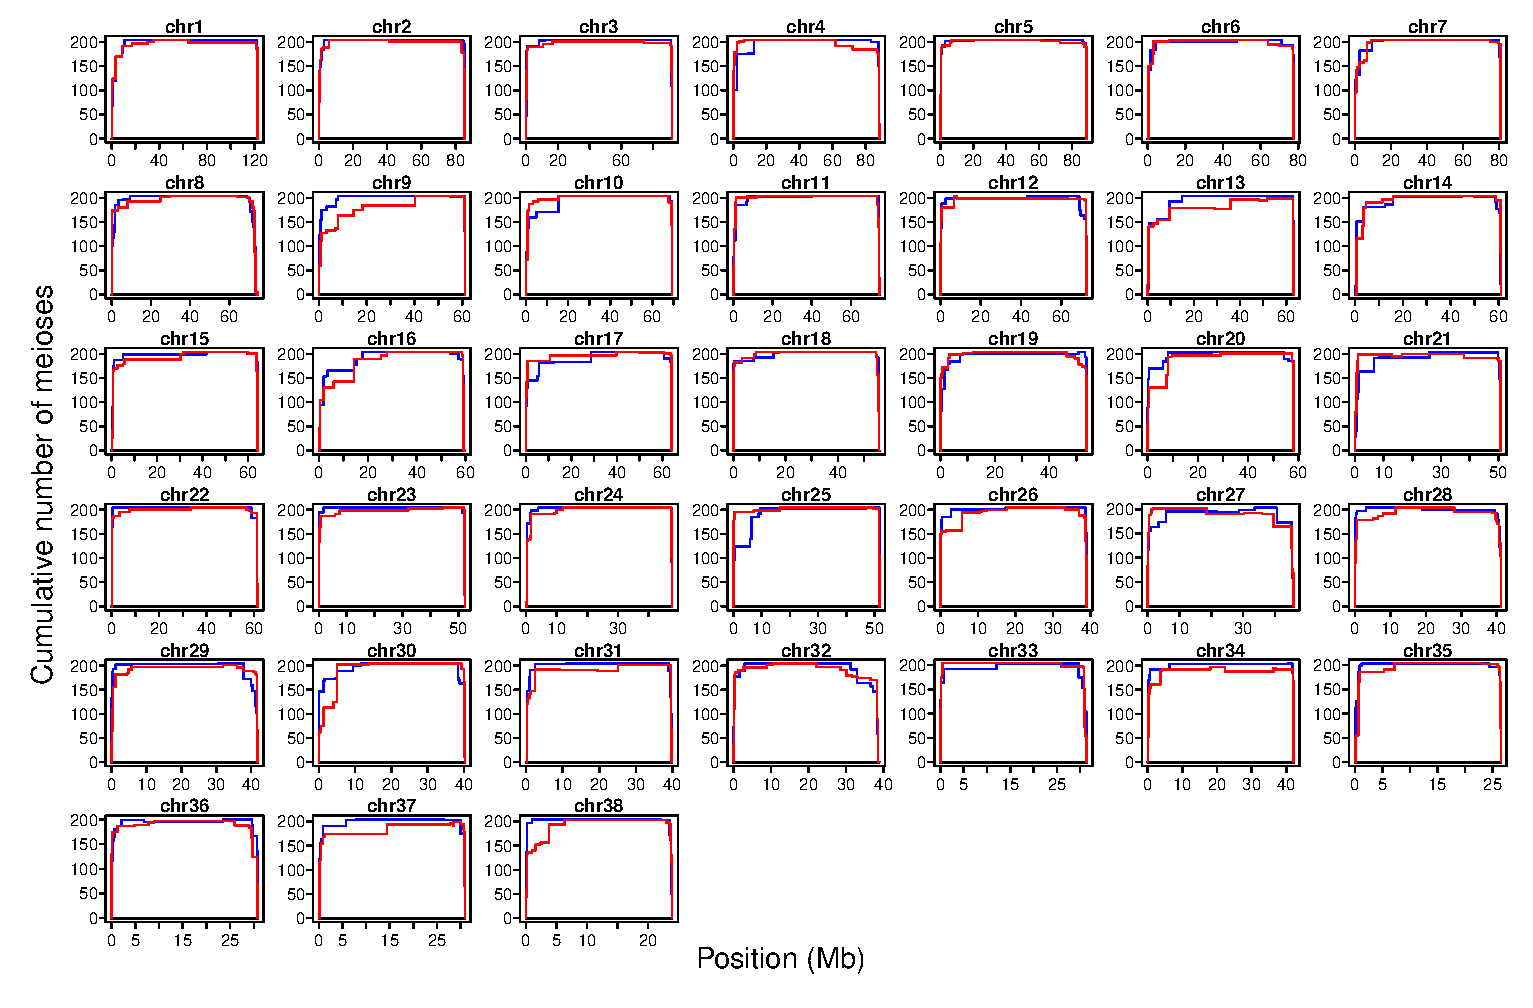
\includegraphics[width=\textwidth]{dogPed/suppfigs/informativeMeioses_step_duohmm2}
    \vspace{-20pt}
    \captionTitle{\textbf{The effective number of meioses as a function of physical position is shown along each chromosome.}}{
    Red curves represent females (n=204), blue curves represent males (n=204). \label{fig:mstep}}
\end{figure}

\begin{figure}[p]
    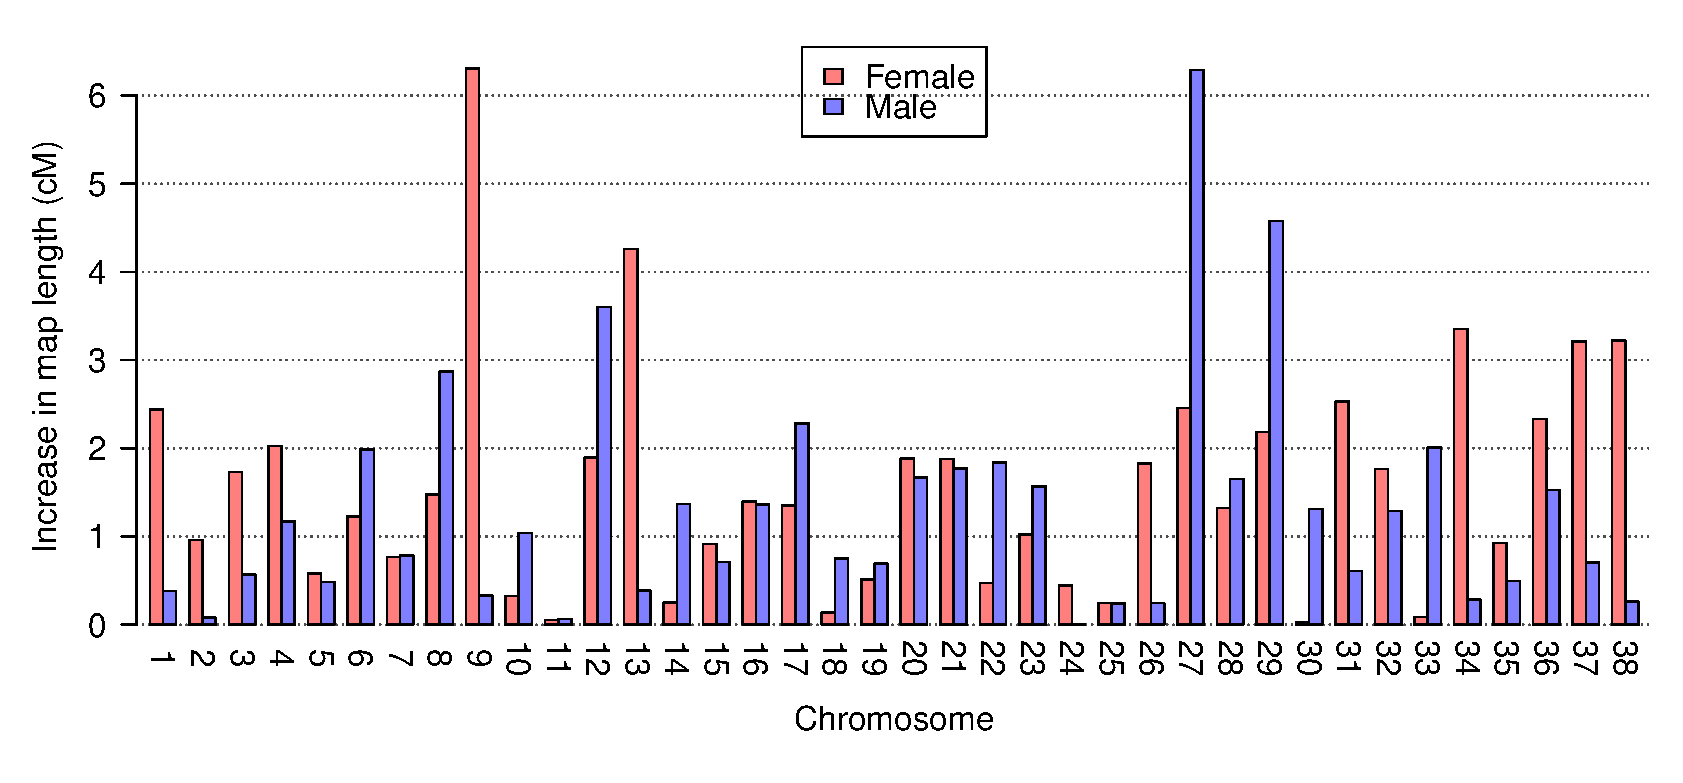
\includegraphics[width=\textwidth]{dogPed/suppfigs/mapLength_increase}
    \vspace{-20pt}
    \captionTitle{\textbf{Increase in map length in each chromosome after accounting for the effective number of meioses.}}{
    Each bar represents the difference in map length after taking into account a reduced number of observable meioses towards chromosome ends compared to the map length calculated using a fixed number of meioses (n=204 for females in red, n=204 for males, blue). \label{fig:mstepIncrease}}
\end{figure}

\begin{figure}[p]
    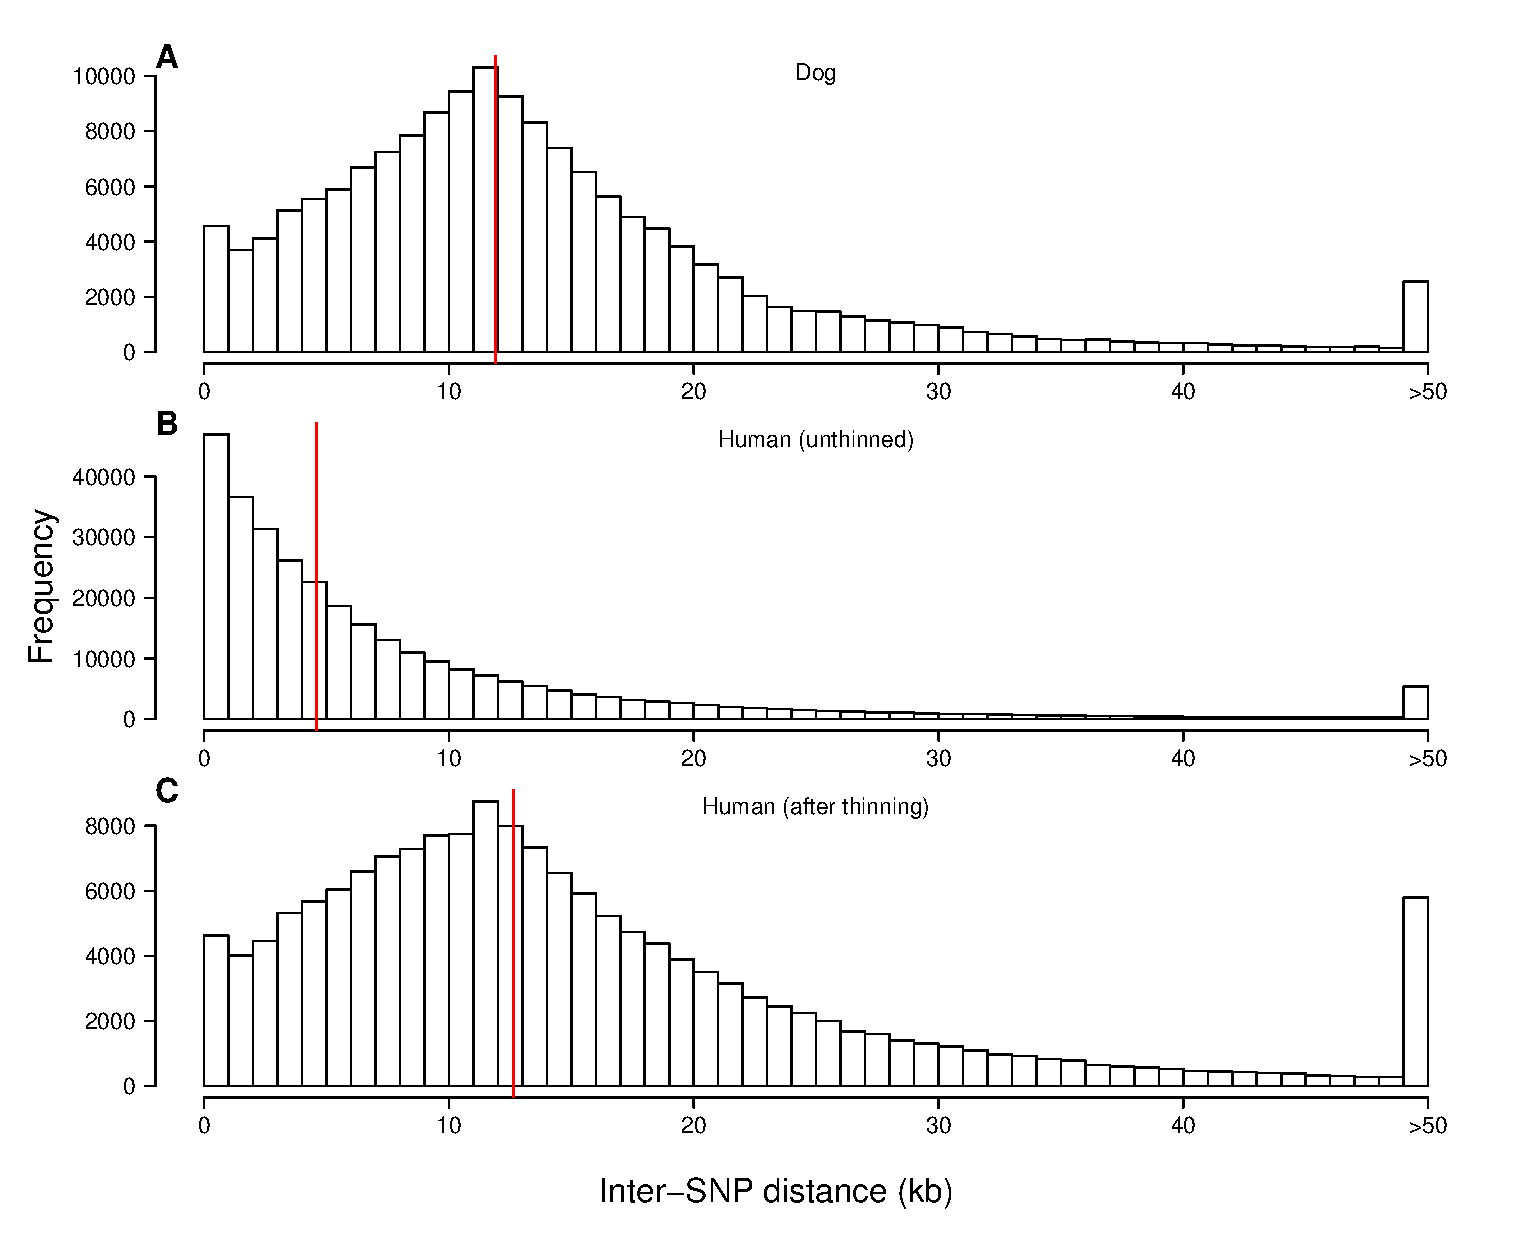
\includegraphics[width=\textwidth]{dogPed/suppfigs/interSNPdist_thinning}
    \vspace{-15pt}
    \captionTitle{\textbf{Distribution of inter-SNP distances in the dog data}}{
    (A), the human data prior to thinning (B), and the human data after the thinning procedure (C). The red line represents the median inter-SNP distance for each distribution.  \label{fig:interSNPdist}}
\end{figure}

\begin{figure}[p]
    \centering
    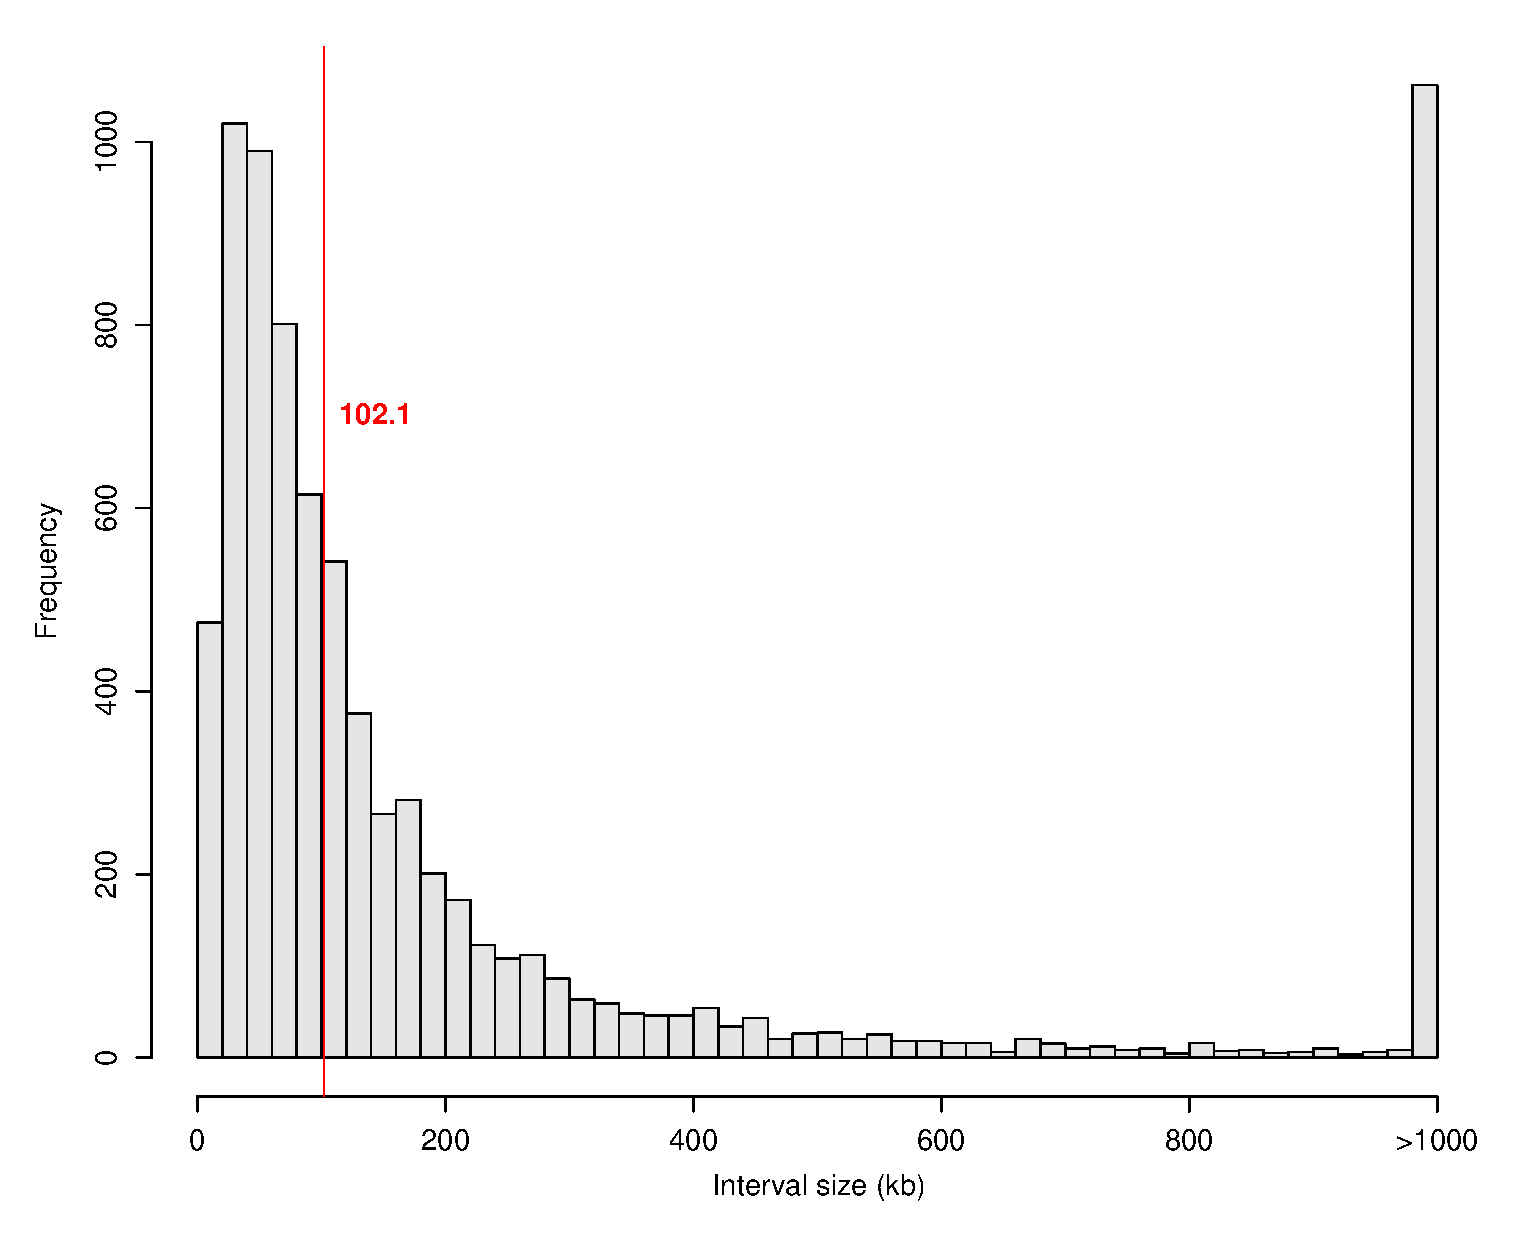
\includegraphics[width=0.5\textwidth]{dogPed/suppfigs/eventWidth_trim_filtered}
    \vspace{-10pt}
    \captionTitle{\textbf{Distribution of crossover interval size.}}{
    The vertical red line represents the median interval size of 102.1 kb.\label{fig:intsize}}
\end{figure}

\begin{figure}[p]
    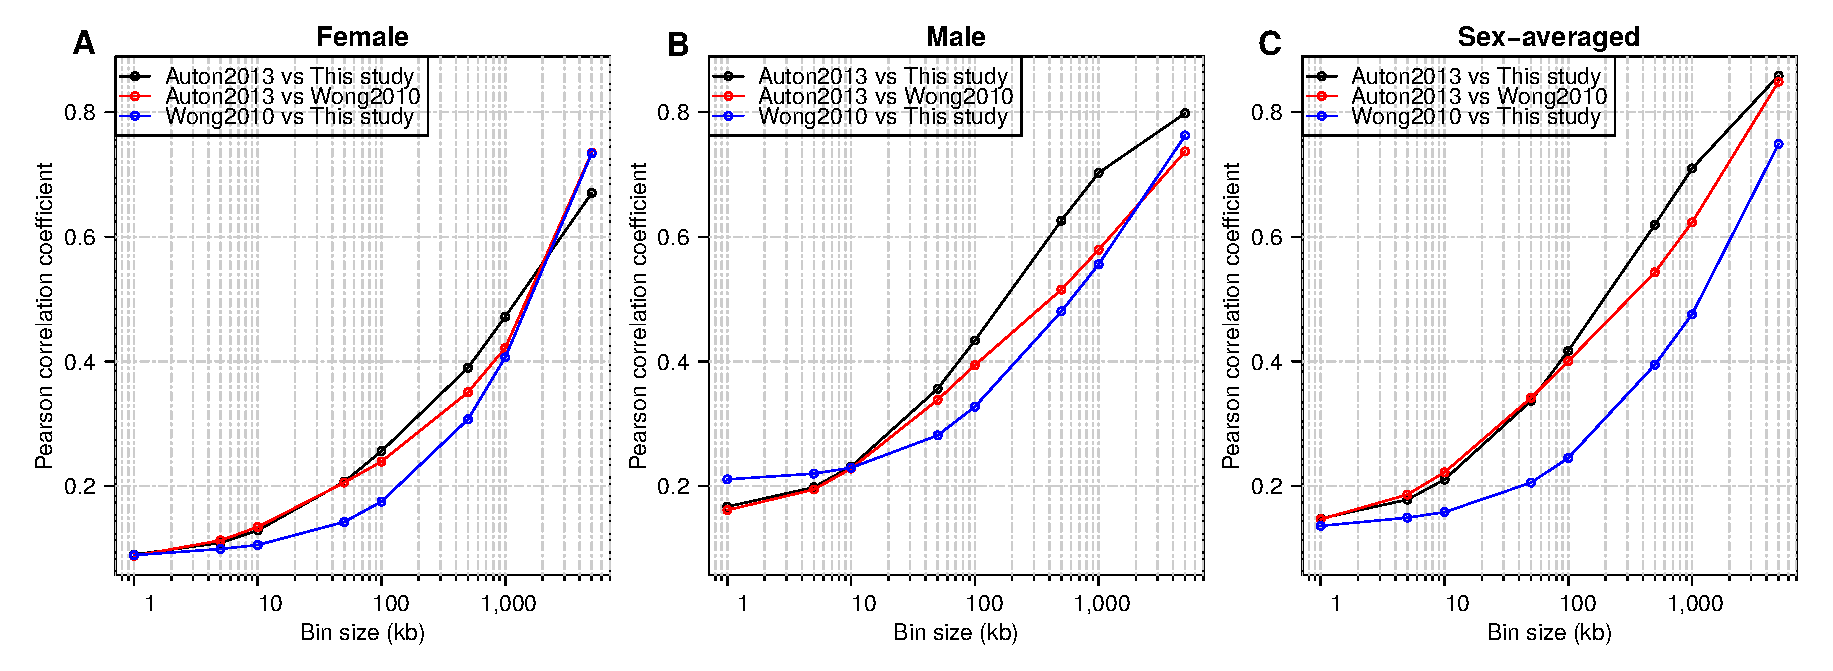
\includegraphics[width=\textwidth]{dogPed/suppfigs/geneticMap_correlations_filtered2}
    \vspace{-20pt}
    \captionTitle{\textbf{Pearson correlation between recombination rates}}{
    estimated from the \citet{Auton2013} LD map, the pedigree maps from \citet{Wong2010}, and this study as a function of scale. \label{fig:mapCor}}
\end{figure}

\begin{figure}[p]
    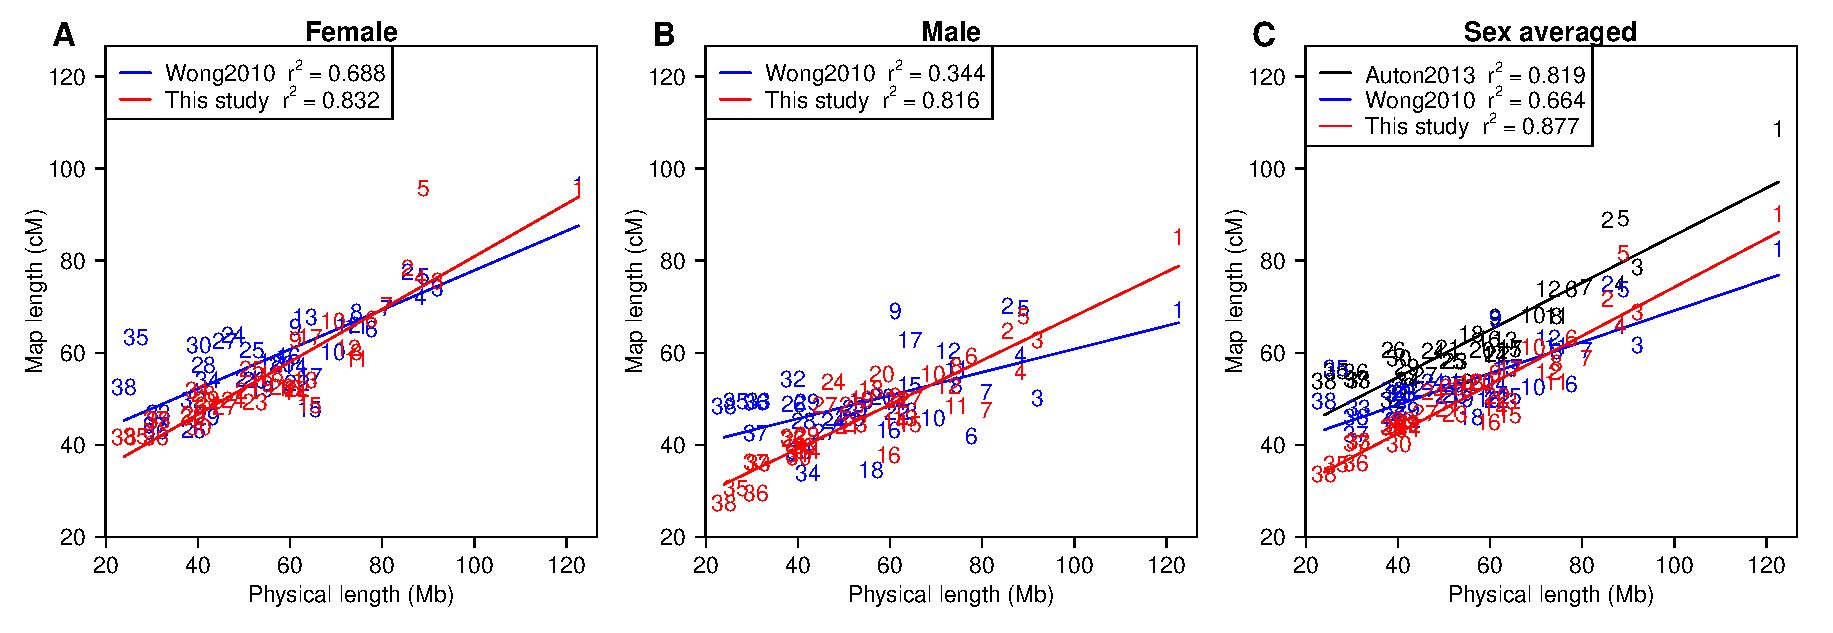
\includegraphics[width=\textwidth]{dogPed/suppfigs/chr_length_relationship_filtered}
    \vspace{-20pt}
    \captionTitle{\textbf{Map length as a function of physical length for each chromosome}}{
    for female (A), male (B), and sex-averaged (C) maps.  Numbers refer to chromosomes with a linear regression line included.   The sex-specific maps are compared to the \citet{Wong2010} pedigree study, the sex-averaged map is additionally compared to the LD map from \citet{Auton2013} (C, in black). \label{fig:mapLength}}
\end{figure}

\begin{figure}[p]
    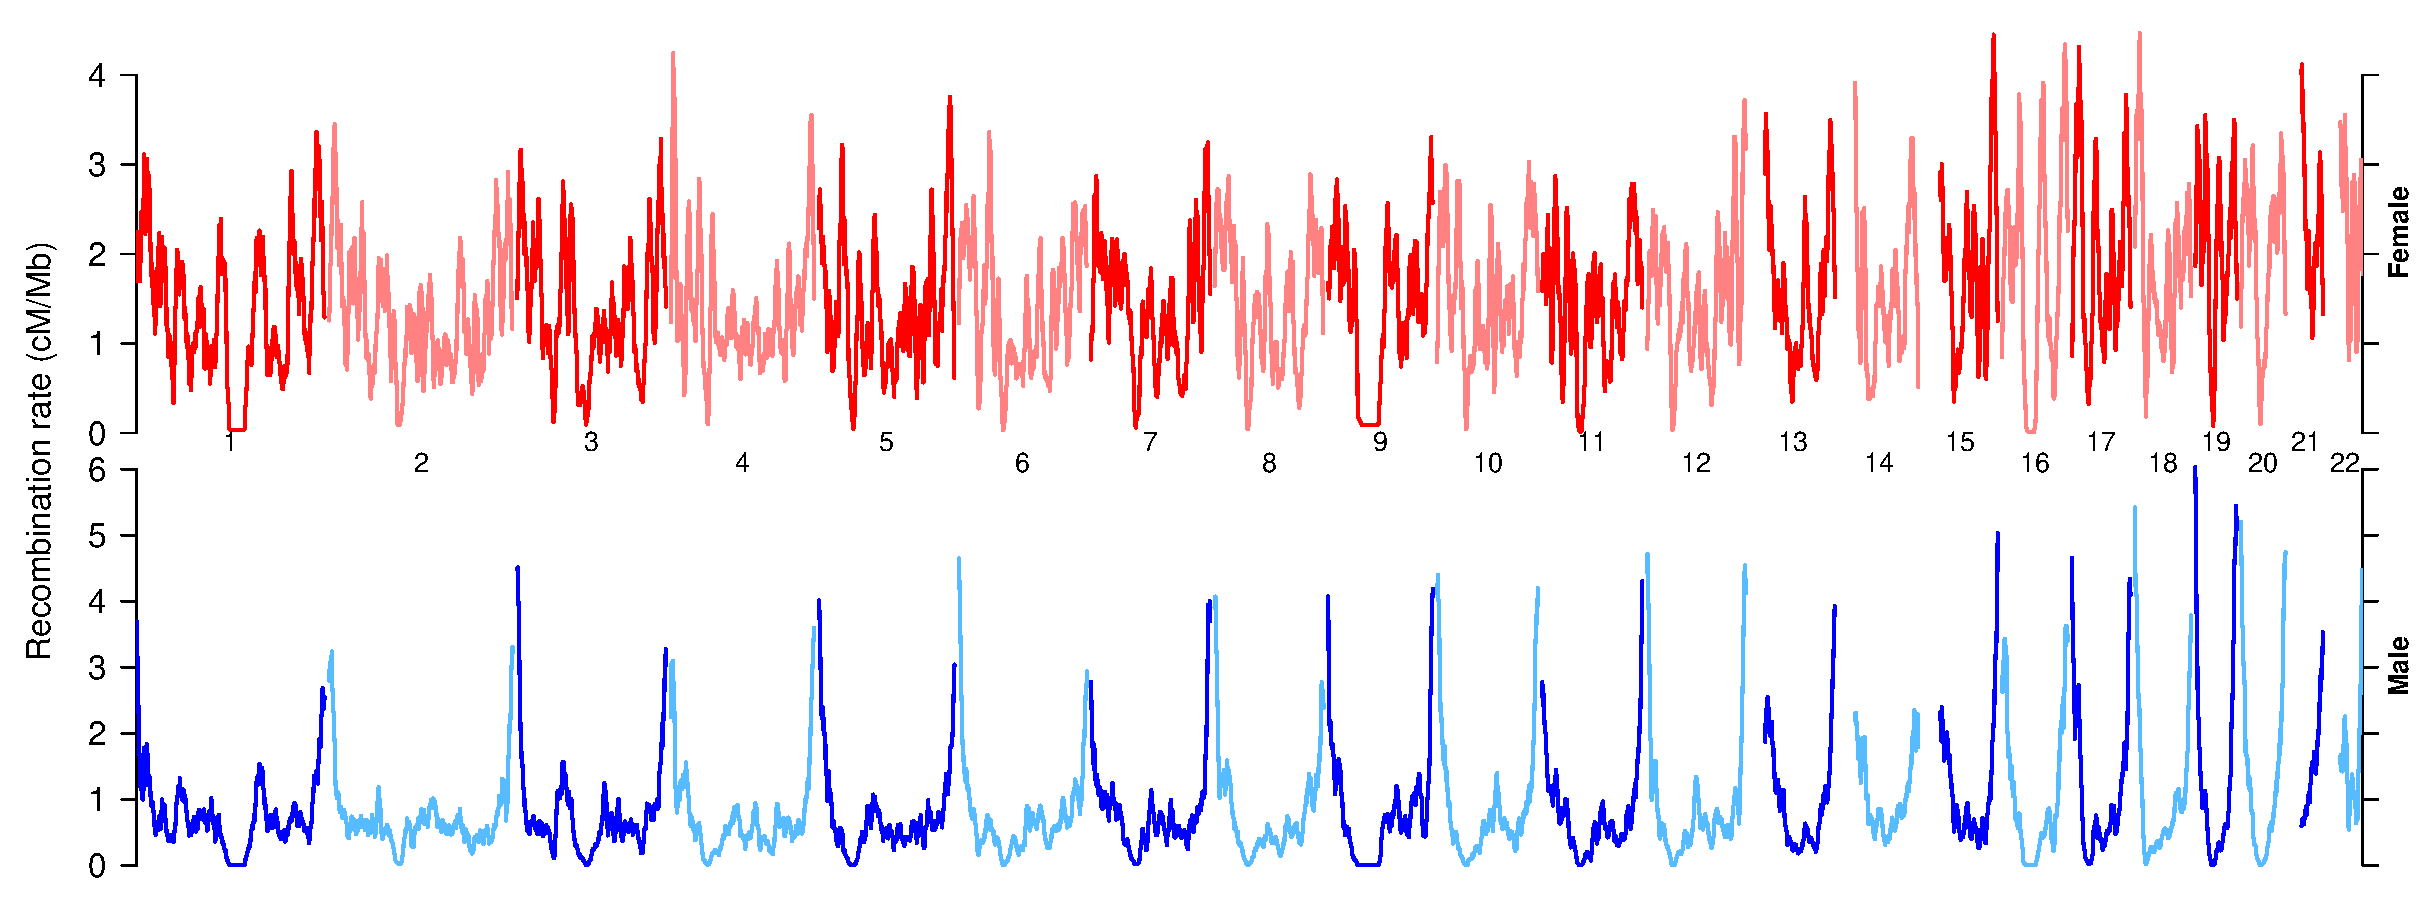
\includegraphics[width=\textwidth]{dogPed/suppfigs/recomb_genome_100kb_k50_human}
    \vspace{-20pt}
    \captionTitle{\textbf{Recombination rate across the human genome}}{
    using the 23andMe genetic maps\cite{Campbell2015}. Female rates are shown in shades of red, male rates in blue shades.  Recombination rates were smoothed at the 5 Mb scale. \label{fig:recombRateHuman}}
\end{figure}

\begin{figure}[p]
    \includegraphics[width=\textwidth]{dogPed/suppfigs/8020plot_supplement}
    \vspace{-15pt}
    \captionTitle{\textbf{SNP density affects the proportion of recombination occupying various proportions of the sequence.}}{
        (A) Human data is shown prior to thinning, alongside data from dogs.  Even without thinning in humans, dogs have a more concentrated distribution of recombination.
        (B) Dog data is shown with the thinned human data.  Here, the most telomeric 15\% (by physical distance) of each chromosome arm has been excluded for both species.  Dog recombination remains more concentrated than humans, although the female and male dog curves have flipped at the 80\% recombination mark, likely as a result of the removal of large amounts of telomeric recombination in males.
        (C) The effects of thinning the SNP framework used to create the genetic maps for the human data. Each curve represents a different marker density, from 300,000 SNPs (red line), to 10,000 (blue line).  Reducing the SNP density moves the curve closer to unity and causes recombination to appear to be more spread out throughout the genome. 
        (D) A reduced set of human and dog data are shown with the chromosome sizes approximately matching.
        Each dog chromosome was paired with a corresponding human chromosome arm of a similar size (within 30 Mb).
        This plot includes dog chromosomes 1 through 28; the remainder were too small to have potential matching human chromosome arms.
    \label{fig:8020supp}}
    \end{figure}

\begin{figure}[p]
    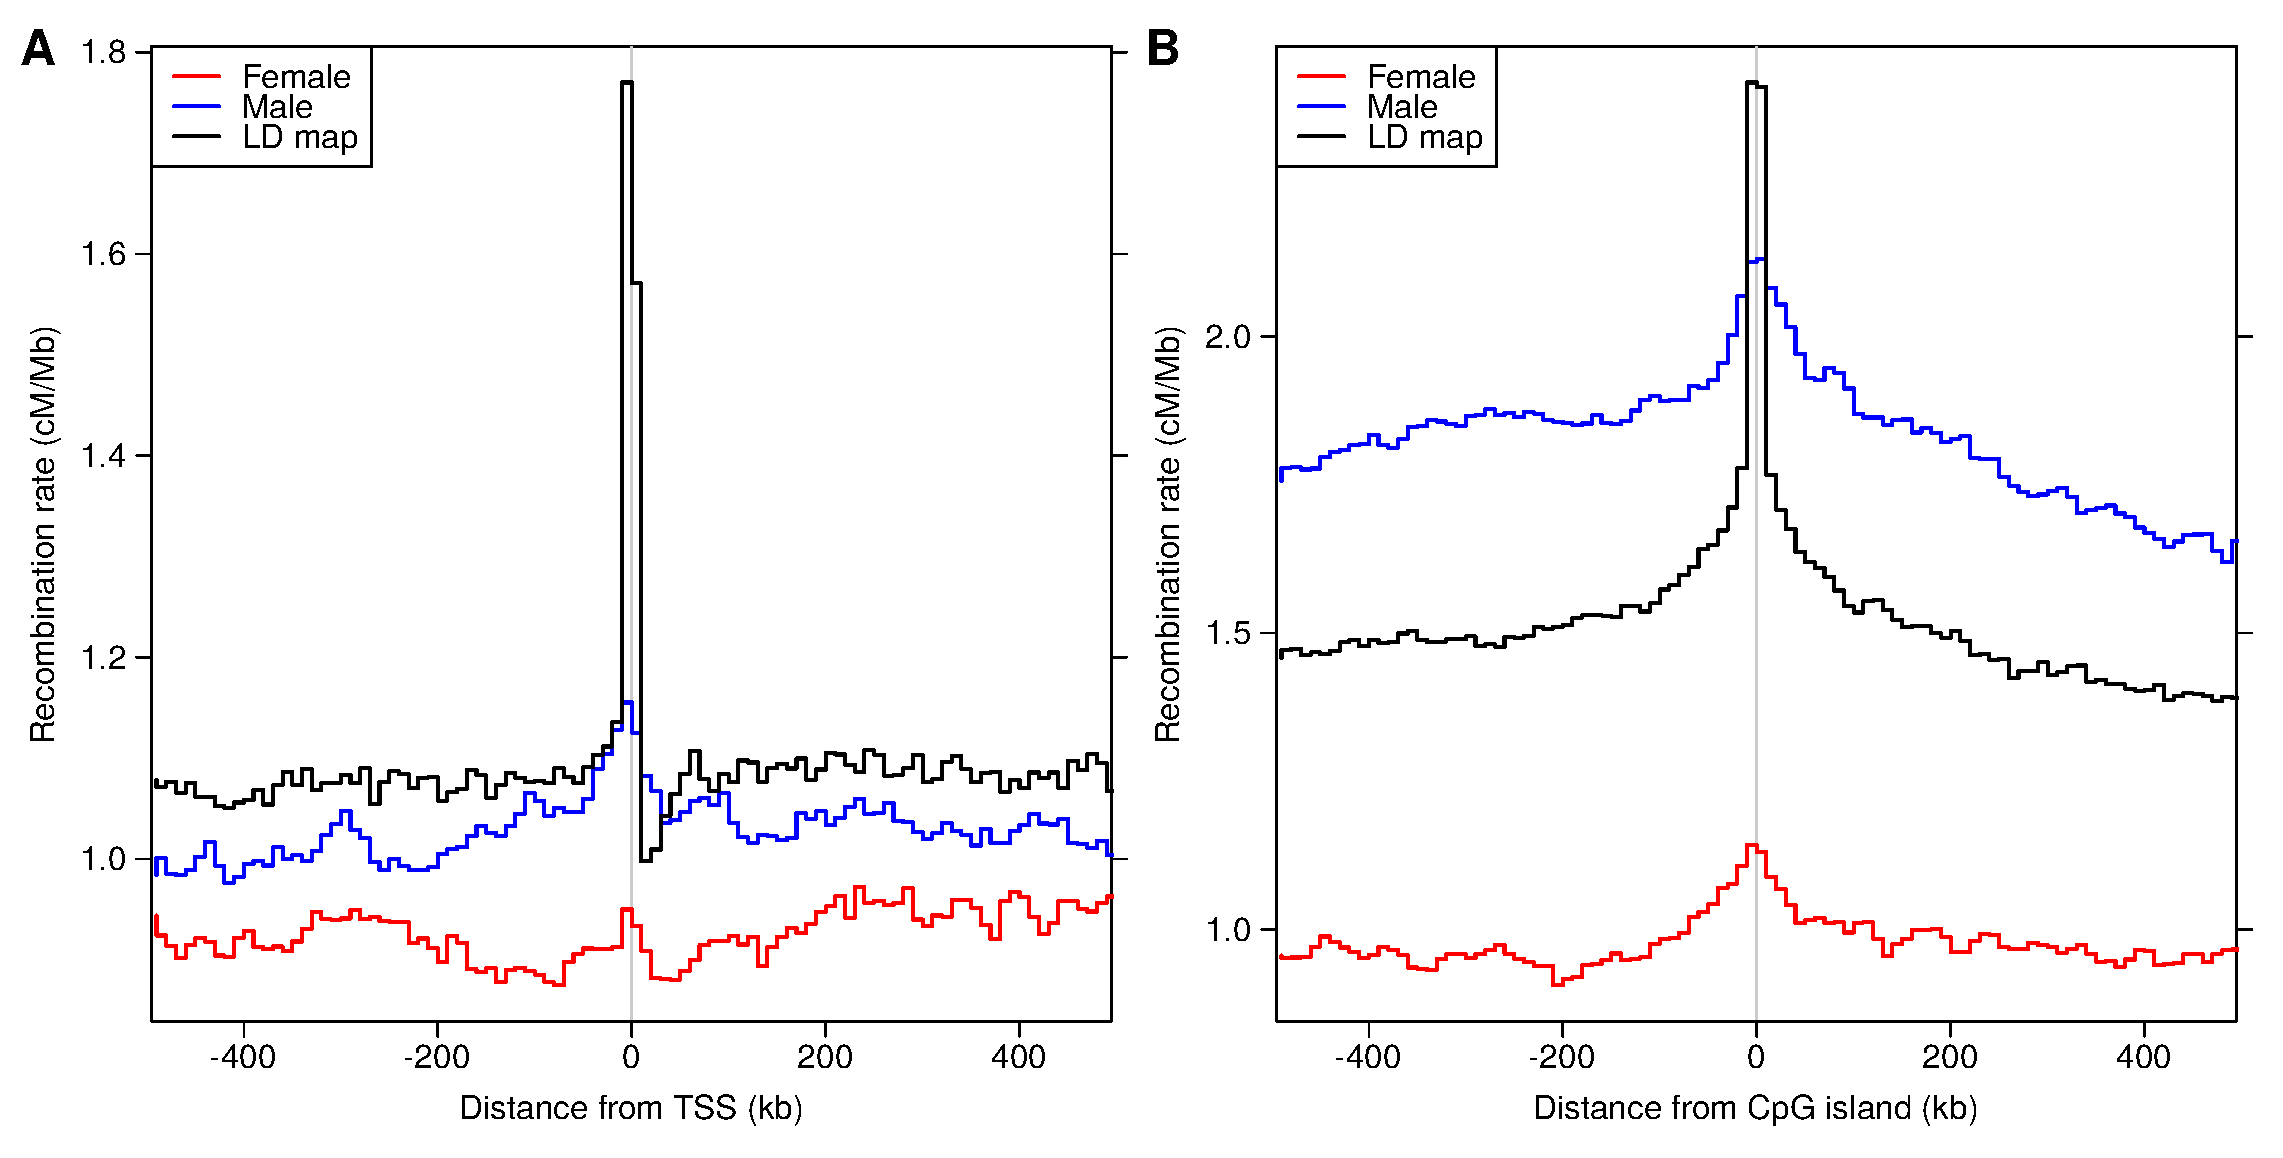
\includegraphics[width=\textwidth]{dogPed/suppfigs/rr_around_TSS-CpG}
    \vspace{-20pt}
    \captionTitle{\textbf{Sex differences in recombination}}{
    around the TSS (A) and CpG islands (B). Female rates are shown red, male in blue.  LD-based estimates\cite{Auton2013} are shown in black.  Recombination rates were estimated in 10 kb windows. \label{fig:genomicFeatures}}
\end{figure}

\begin{figure}[p]
    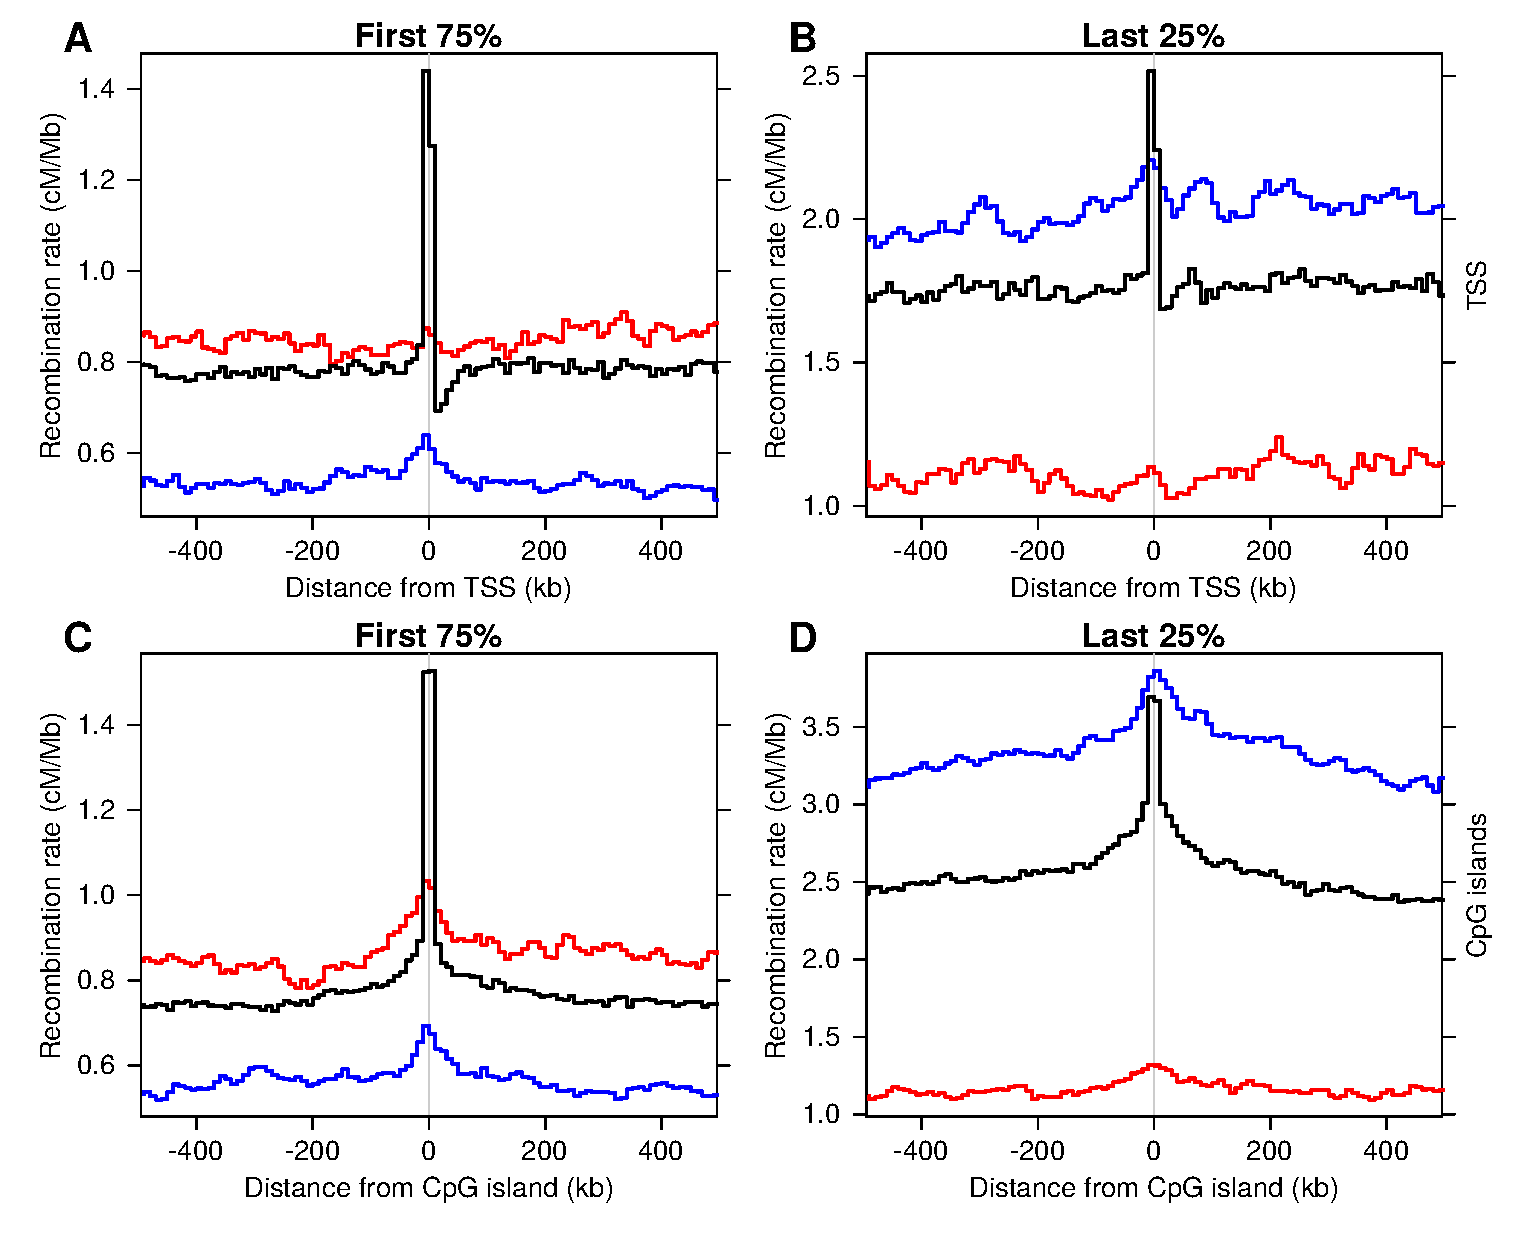
\includegraphics[width=\textwidth]{dogPed/suppfigs/rr_around_TSS-CpG_split}
    \vspace{-15pt}
    \captionTitle{\textbf{Recombination around TSS and CpG islands partitioned by chromosome position.}}{ 
    Male rates are in blue, female in red, rates from the LD map in black. Rates were estimated in 10 kb bins.  Rates were estimated for each feature by taking the centromeric 75\% (A and C) and telomeric 25\% (B and D) of each chromosome separately. \label{fig:TSScpgSplit}}
\end{figure}

\begin{figure}[p]
    \centering
    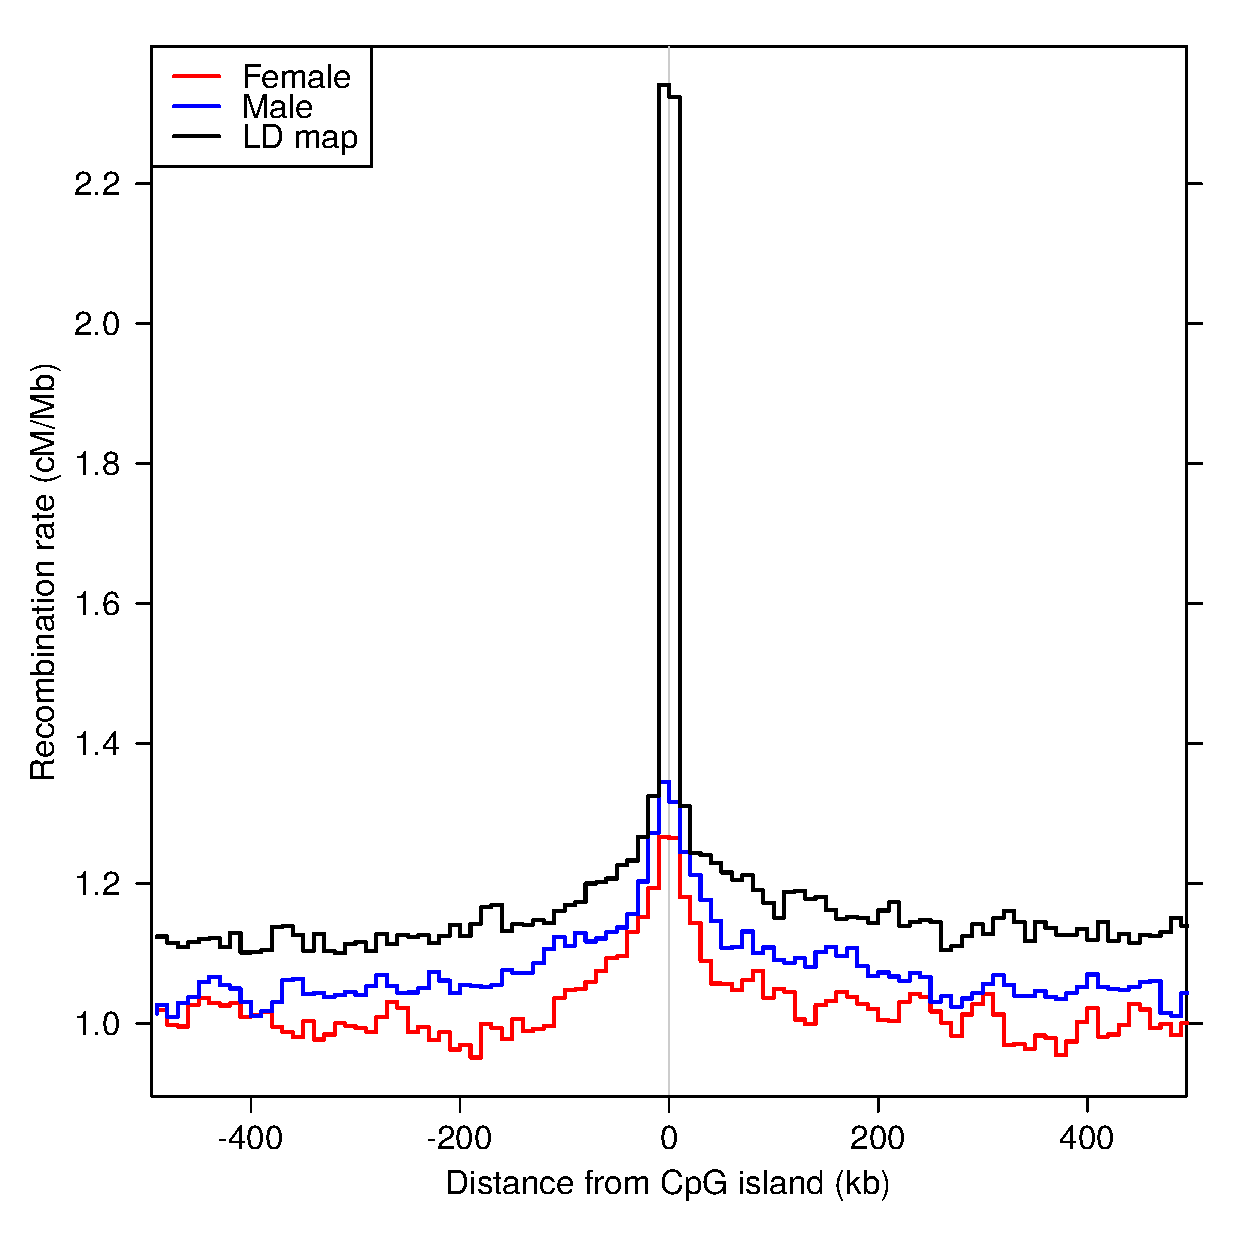
\includegraphics[width=0.6\textwidth]{dogPed/suppfigs/rr_around_CpG_thinned}
    \vspace{-10pt}
    \captionTitle{\textbf{Recombination around a thinned subset of CpG islands.}}{
    Male rates are in blue, female in red, rates from the LD map in black.  Rates were estimated in 10 kb bins.  CpG islands were thinned to a uniform distribution by keeping a maximum of 5 per non-overlapping 500 kb window. \label{fig:cpgThinned}}
\end{figure}

\clearpage

\begin{figure}[p]
    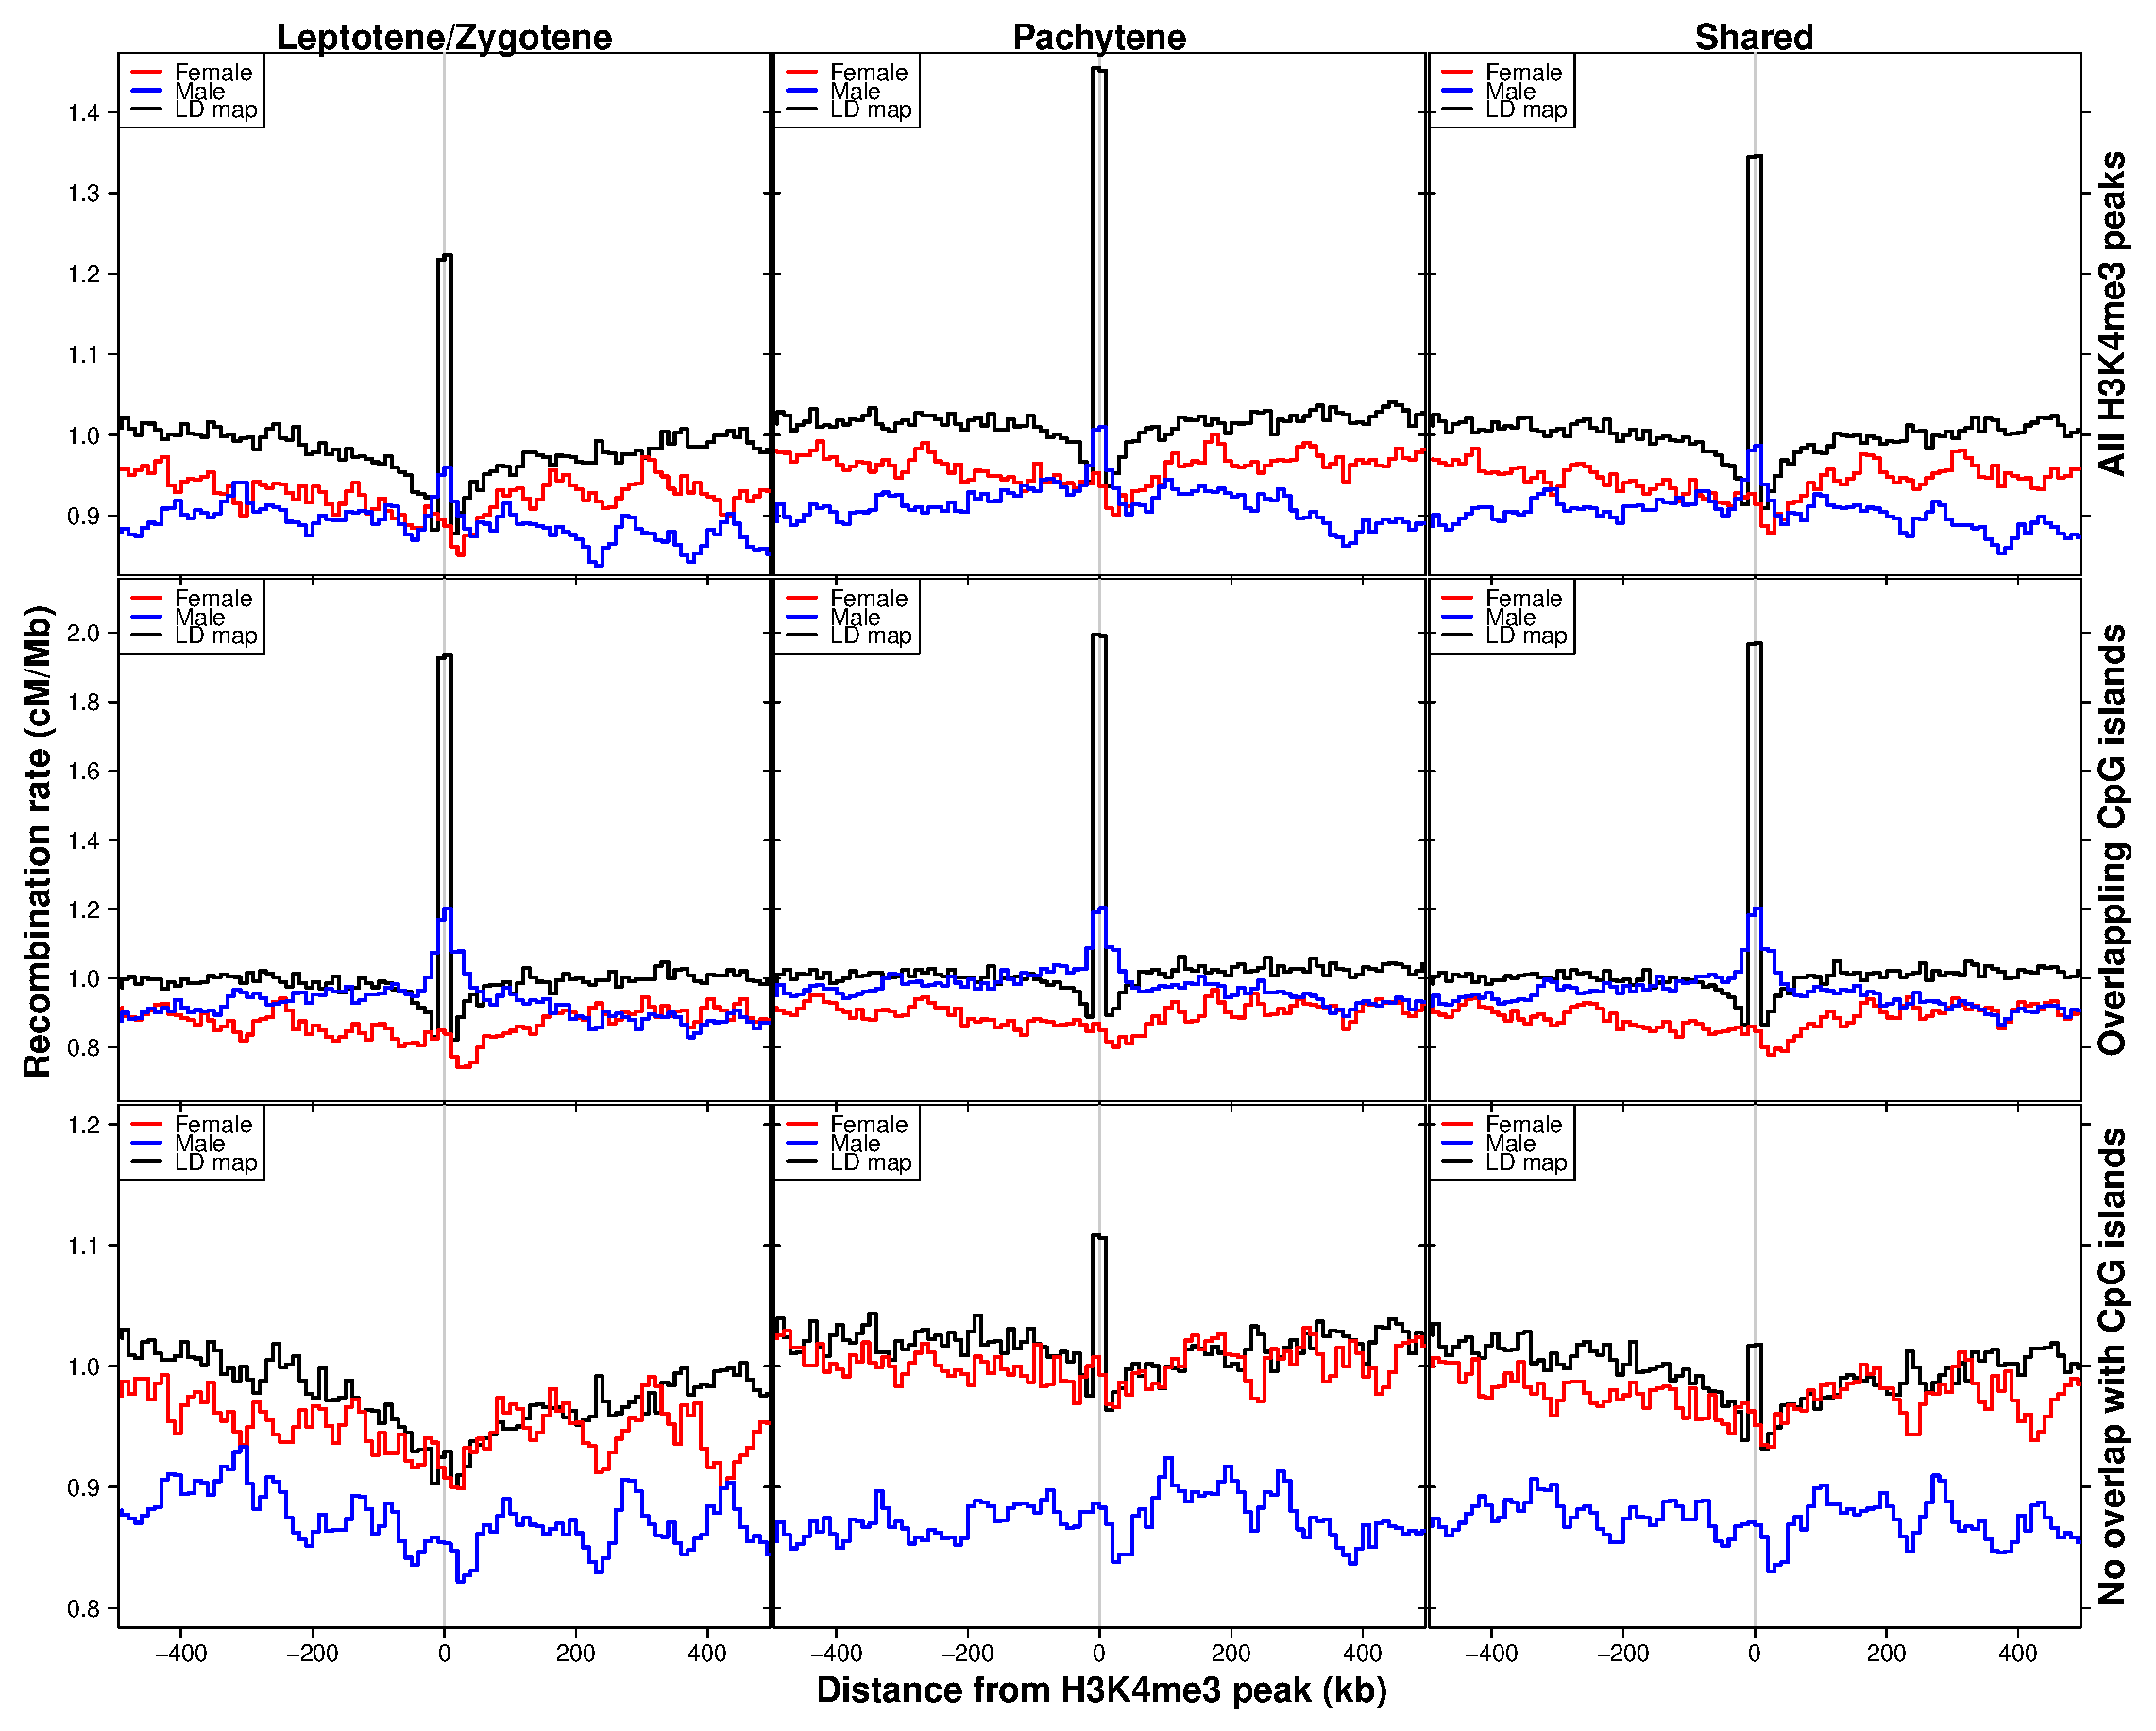
\includegraphics[width=\textwidth]{dogPed/suppfigs/rr_around_H3K4me3_splitCpG}
    \vspace{-20pt}
    \captionTitle{\textbf{Recombination rate around H3K4 trimethylation marks found in dog spermatocytes of varying stages}}{ 
        Male rates are shown in blue, female in red, and rates from the LD-based map in black.
        %The left column of plots shows peaks in early stages of meiosis (leptotene/zygotene, n=28,303), the middle column pachytene (n=32,718), and the right column the union of all peaks (n=61,021).
        The left column of plots shows peaks in early stages of meiosis (leptotene/zygotene), the middle column pachytene, and the right column the union of all peaks.
        Similarly, the top row includes all peaks, while the middle and bottom rows show peaks with and without overlap with CpG islands, respectively. Rates were estimated in 10 kb bins for all plots.
    \label{fig:H3K4panel}}
\end{figure}

\begin{figure}[p]
    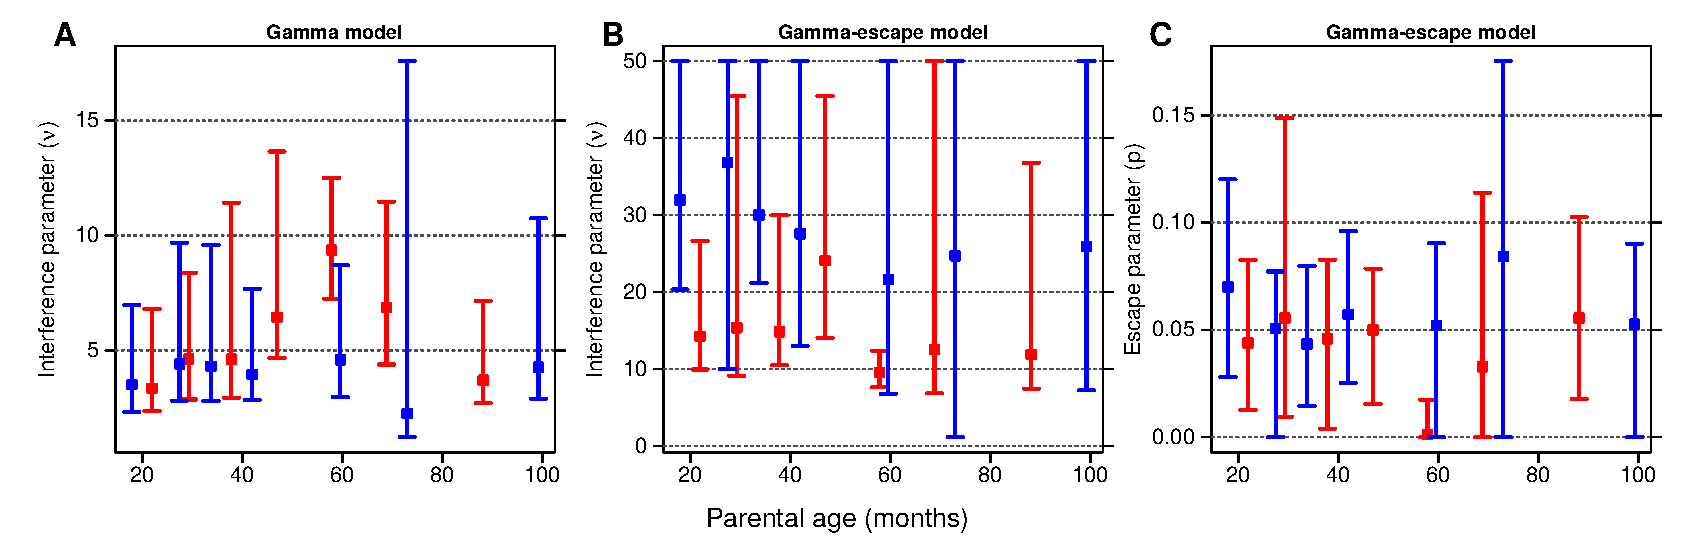
\includegraphics[width=\textwidth]{dogPed/suppfigs/interferenceParameters_byAge}
    \vspace{-20pt}
    \captionTitle{\textbf{Estimates of crossover interference parameters in the dog genome as a function of age.}}{
       Dog meioses were partitioned into 7 approximately equal sized bins on the basis of parental age at birth.
       Interference strength for the simple gamma model is shown in A.
       The parameters for the Housworth-Stahl gamma-escape model are shown in B (interference strength) and C (escape).
       Males are shown in blue and females in red.
       The error bars represent a 95\% confidence interval estimated from 100 bootstrap iterations. \label{fig:cointGenomeAge}}
\end{figure}

\begin{figure}[p]
    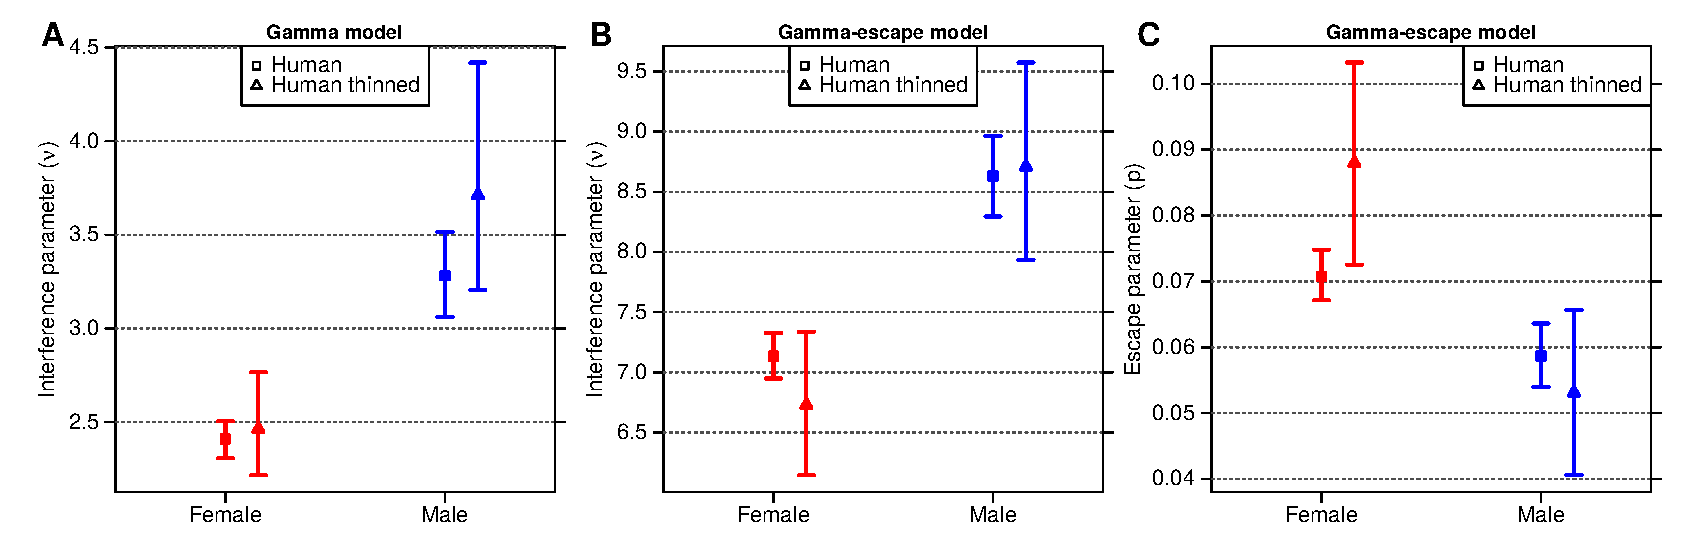
\includegraphics[width=\textwidth]{dogPed/suppfigs/interferenceParameters_genome_thinned}
    \vspace{-20pt}
    \captionTitle{\textbf{Estimates of crossover interference parameters in the human genome.}}{
       Here, the human data is thinned according to the procedure outlined in the Methods section, reducing the meiosis count and number of SNPs to more closely resemble what is found in dogs.
       Interference strength for the simple gamma model is shown in A.
       The parameters for the Housworth-Stahl gamma-escape model are shown in B (interference strength) and C (escape).
       Males are shown in blue and females in red.
       Estimates for the full resolution human data are shown in boxes, and the thinned human data in triangles.
       The error bars represent a 95\% confidence interval estimated from 1000 bootstrap iterations. \label{fig:cointGenomeThin}}
\end{figure}

\beginmain
